\documentclass[preprint,3p,review,12pt]{elsarticle}

\journal{Progress in Oceanography}

%% The graphicx package provides the includegraphics command.
\usepackage{graphicx}
%% The amssymb package provides various useful mathematical symbols
\usepackage{amssymb}
%% The amsthm package provides extended theorem environments
%% \usepackage{amsthm}

\usepackage{natbib}

%% The lineno packages adds line numbers. Start line numbering with
%% \begin{linenumbers}, end it with \end{linenumbers}. Or switch it on
%% for the whole article with \linenumbers after \end{frontmatter}.
\usepackage{lineno}

\usepackage{floatpag} % safe to include before "float" package.
% ^^^ by default, it moves the page number to the top on figure-only pages.
%\floatpagestyle{empty} % Prevents page numbering on figure-only pages.

\usepackage{float}
% \usepackage{endfloat}
\usepackage{adjustbox}

% % Give an extra option to the rotating package,
% % which is loaded in ametsoc.cls, I think (Ryo).
\usepackage{rotating}
\PassOptionsToPackage{figuresright}{rotating}

% %--- for sidewaysfigure in "rotating" package:  Ryo (14 June 2018) ---
% % The endfloat package messes it up. For sidewaysfigure to
% % play nicely with endfloat, the following additional
% % declaration(s) are necessary.
% \DeclareDelayedFloatFlavor{sidewaysfigure}{figure}
% \DeclareDelayedFloatFlavor{sidewaystable}{table}

% %Citations should be of the form ``author year''  not ``author, year''
\bibpunct{(}{)}{;}{a}{}{,}

% %% Earl's stuff
\usepackage{csquotes} % Ryo (13 June 2018)
%\usepackage{upgreek} % for the upright tau
% \usepackage{silence}
\usepackage{siunitx}
\usepackage{amsmath}
\usepackage{url}


% %--- some convenience macros ---
\newcommand{\citepos}[1]{\citeauthor{#1}'s \citeyearpar{#1}}
\renewcommand{\Vec}[1]{\mathbf{#1}}
 
%  % Sometimes we want to say "700-m" as in "700-m isobath".
%  % Here is a variant of the \SI{}{} command for that.
%  % https://tex.stackexchange.com/questions/228511/how-to-write-hyphen-between-number-and-unit-in-an-attribute-30-s-acquisition-w
\newcommand{\SIadj}[2]{\SI[number-unit-product={\text{-}}]{#1}{#2}}

% NOTE: We are no longer using these!!
\usepackage[authormarkup=none, draft]{changes}
% \usepackage[authormarkup=none, final]{changes}

% Earl
\definechangesauthor[name={Earl Duran}, color=red]{erd}
\newcommand{\adderd}[1][]{\added[id=erd,remark={#1}]}
\newcommand{\delerd}[1][]{\deleted[id=erd,remark={#1}]}
\newcommand{\reperd}[1][]{\replaced[id=erd,remark={#1}]}
\newcommand{\comerd}[1]{\delerd[#1]{COMMENT}}

% Helen
\definechangesauthor[name={Helen Phillips}, color=blue]{hp}
\newcommand{\addhp}[1][]{\added[id=hp,remark={#1}]}
\newcommand{\delhp}[1][]{\deleted[id=hp,remark={#1}]}
\newcommand{\rephp}[1][]{\replaced[id=hp,remark={#1}]}
% Ryo
\definecolor{darkergreen}{rgb}{0,0.7,0}
\definechangesauthor[name={Ryo Furue}, color=darkergreen]{rf}
\newcommand{\addrf}[1][]{\added[id=rf,remark={#1}]}
\newcommand{\delrf}[1][]{\deleted[id=rf,remark={#1}]}
\newcommand{\reprf}[1][]{\replaced[id=rf,remark={#1}]}
%\newcommand{\comrf}[1]{\textcolor{darkergreen}{[#1]}}
\newcommand{\comrf}[1]{\delrf[{#1}]{COMMENT}}

% Paul
\definechangesauthor[name={Paul Spence}, color=orange]{ps}
\newcommand{\addps}[1][]{\added[id=ps,remark={#1}]}
\newcommand{\delps}[1][]{\deleted[id=ps,remark={#1}]}


% % Ryo: ad-hoc fix for vertical spacing in footnotes.
% % Delete the following settings in the version you submit to AMS.
% % FROM HERE >>>>>>>>>>
% \renewcommand{\baselinestretch}{1} % Undo the double-spacing done in ametsoc.cls
% \usepackage{setspace} %% A better way to double-space the document.
% \setstretch{2.5}      %% For one thing, it doesn' mess with footnotes.
% % <<<<<<<< TO HERE.

% % Ryo: Fix the overly-stylized mathcal back to LaTeX's original.
% % The fancy mathcal is due to the mathptmx package, which is loaded in ametsoc.cls .
% % See https://tex.stackexchange.com/questions/67881/resetting-mathcal-font-to-default
% % I'm sure AMS wouldn't mind this change because they accepted my LaTeX source
% % that didn't use ametsoc.cls .
\DeclareMathAlphabet{\mathcal}{OMS}{cmsy}{m}{n}

% % Merely for convenience
\newcommand{\dg}{$^{\circ}$}
\newcommand{\sub}[1]{_{\text{#1}}}

\DeclareSIUnit\year{yr}

\begin{document}
\begin{frontmatter}

\title{Southern Australia Current System based on a gridded hydrography and a high-resolution model}

\author[label2]{Earl R. Duran\corref{cor1}}
\ead{earl.r.duran@gmail.com}
\author[label3,label4]{Helen E. Phillips}
\author[label5]{Ryo Furue}
\author[label2,label4]{Paul Spence}
\author[label3,label4,label6,label7]{Nathaniel L. Bindoff}

\address[label2]{Climate Change Research Centre (CCRC), University of New South Wales, Sydney, NSW 2052 Australia}
\address[label3]{Institute for Marine and Antarctic Studies (IMAS), Hobart, Tasmania, Australia}
\address[label4]{ARC Centre of Excellence for Climate Extremes (CLEX)}\address[label5]{Japan Agency for Marine-Earth Science and Technology (JAMSTEC), Yokohama, Japan}
\address[label6]{Commonwealth Scientific and Industrial Research Organisation (CSIRO)}
\address[label7]{Antarctic Climate and Ecosystems Cooperative Research Centre (ACE CRC), Hobart, Tasmania, Australia}

\cortext[cor1]{Climate Change Research Centre, Level 4 Mathews Building, The University of New South Wales, Sydney NSW 2052}

\begin{abstract}
We describe the Southern Australia Current System's annual-mean structure, transport budget and currents coupling along the southern Australian shelves. The system contains eastward Shelf Break Currents (SBC), which is a series of shallow currents over the shelf break including the Leeuwin Current Extension, the South Australian Current and the Zeehan Current; and a counter-flowing westward Flinders Current (FC) found both offshore of, and underneath, the SBC\@.
In this work, we use a climatological hydrography gridded at high resolution and a high resolution oceanic general circulation model simulation forced by an atmospheric climatology to describe the system.

The westward FC has an annual-mean speed up to \SI{10}{\centi\meter\per\second} and a dual structure with (1) the slope-FC, a small slope-trapped part near 600m depth, which is an undercurrent to the SBC; and (2) the offshore-FC, a large deep-reaching, surface-intensified part located offshore of the SBC\@.
Where the continental shelf is slanted (east of \ang{132}E), the annual-mean FC is a weak westward flow disconnected from the Tasman Leakage, which is a westward outflow south of Tasmania transporting \SI{11}{Sv} offshore.
The FC is fed by horizontal onshore flows across the South Australian Basin, where nearly 80\% of these flows occur where the continental shelf is zonal (west of \ang{132}E), resulting in strongest annual-mean FC transport of \SI{12.3}{Sv} at Cape Leeuwin, the southwestern limit of Australia.
To the south of the FC, a deep-reaching eastward jet may be an expression of the Albany High's southern branch and a recirculated source water for the FC.

The eastward SBC are continuous flows with annual-mean speed up to \SI{20}{\centi\meter\per\second} located in the upper \SI{250}{\meter}. A strong annual-mean downwelling occurs from the SBC into the slope-FC where the slope is steep and may be important in maintaining the slope-FC\@.
The annual-mean Leeuwin Current Extension transport decreases from \SI{1.1}{Sv} as it rounds Cape Leeuwin to \SI{0.1}{Sv} at the western edge of the Great Australian Bight due to strong downwelling and offshore exports near Cape Leeuwin. 
East of Cape Leeuwin and along the zonal shelf, the South Australian Current transport is steady due to onshore flows balanced out by downwelling exports. Along the slanted shelf, the onshore flows are stronger than downwelling exports and result in an increased Zeehan Current transport up to \SI{0.4}{Sv} eastward south of Tasmania.

We find that the SBC and offshore-FC are coupled through onshore Ekman drift and that the SBC and slope-FC are coupled through downwelling. 
The combined effect of the SBC--offshore-FC horizontal pair and SBC--slope-FC vertical pair is a conversion of widespread northward Ekman drift into downwelling with little impact on the eastward SBC transport. In contrast, the onshore flows feeding into the FC are largely converted into increasing westward FC transport.
Even though the Leeuwin Current System off western Australia and the Southern Australia Current System are fed by different onshore transports, namely a pressure gradient-driven geostrophic transport off western Australia and a wind-driven Ekman drift off southern Australia, the annual-mean circulation of the two systems are remarkably similar.

An overview of the system's seasonality shows the strength of the SBC and FC vary in opposite phase. In summer, when the winds are upwelling favourable, the SBC are weaker and partly reversed (to westward). In autumn, the winds become downwelling favourable and the FC is weaker and partly reversed (to eastward). In contrast, the Leeuwin Current System persists annually. The balance mechanism maintaining the seasonal opposition in intensity between the SBC and FC is unknown and warrants further research.
\end{abstract}

\begin{keyword}
Southern Australia Current System \sep Shelf break currents \sep Flinders Current \sep Transport budget
\end{keyword}

\end{frontmatter}

\linenumbers

\section{Introduction} \label{Introduction}
\subsection{Australia's Northern Boundary Currents} \label{Australia's Northern Boundary Currents}
The southern continental margin of Australia hosts a unique northern boundary circulation which transports waters between Cape Leeuwin, the southwest corner of Australia, and South East Cape, the southern tip of Tasmania (Fig.\,\ref{f01_fig1_}). Other major boundary currents typically transport water meridionally. The Leeuwin Current flows southward along western Australia and joins the eastward-flowing shelf break currents along southern Australia to form a \SI{5500}{km}-long boundary current starting from North West Cape (\ang{21.8}S) off western Australia to South East Cape, Tasmania (\ang{43.6}S). These surface currents represent the longest boundary circulation in the world \citep{Middleton2007,Ridgway2004}.
%
\begin{figure}[h]
\noindent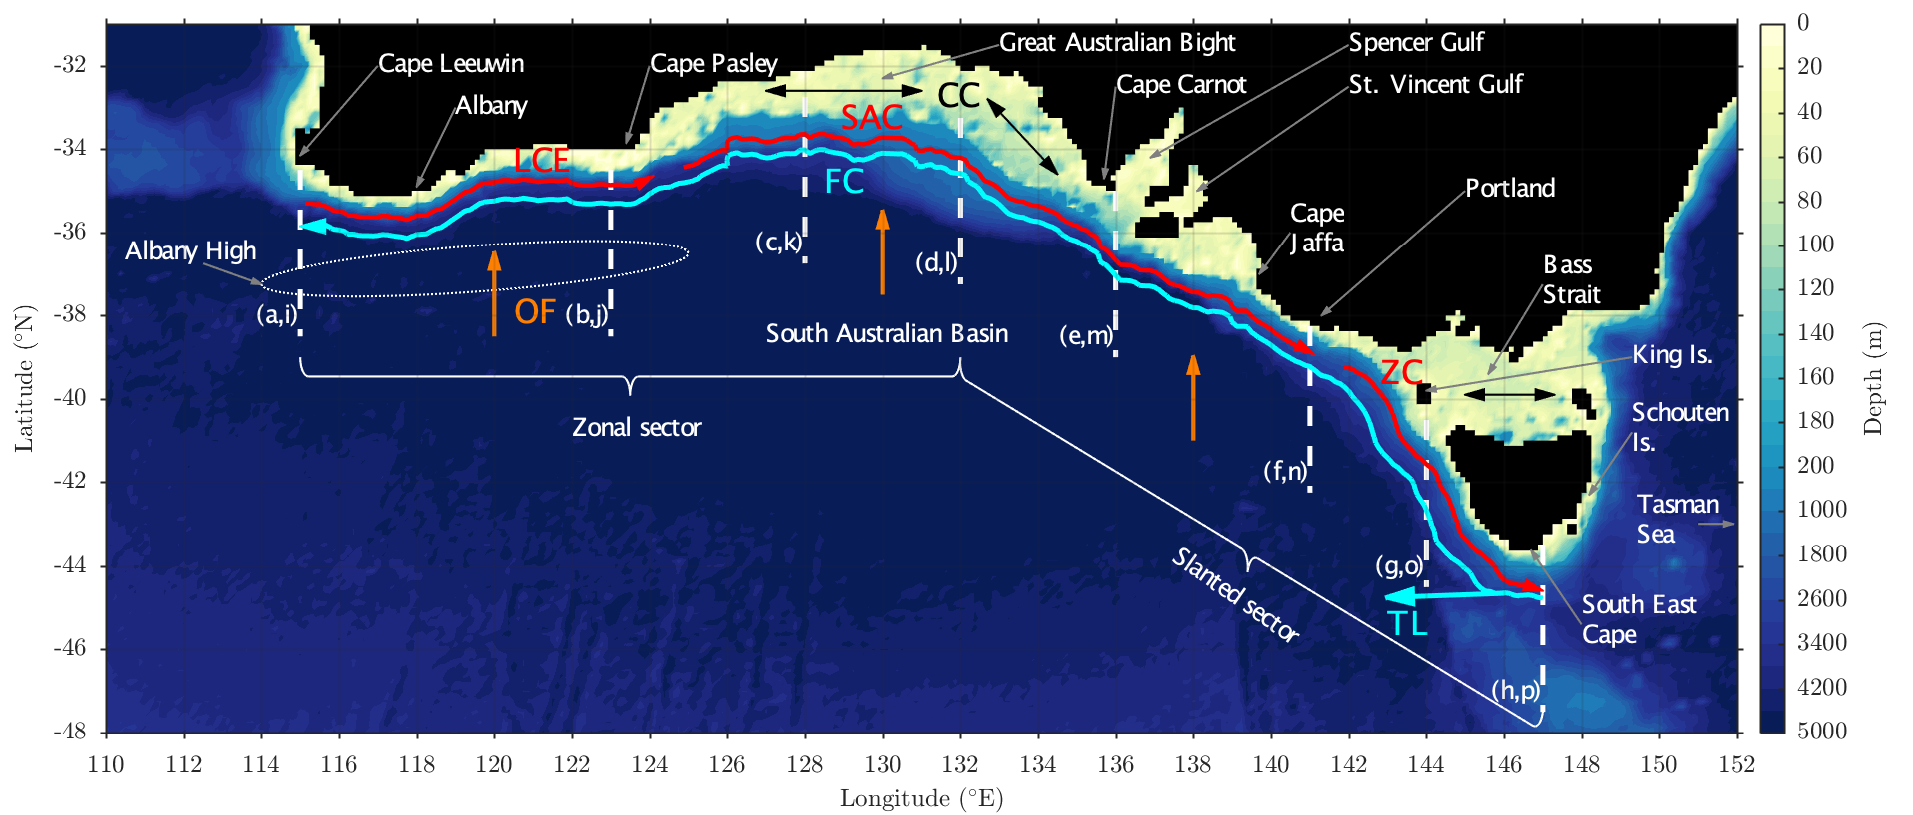
\includegraphics[width=1\textwidth, height=0.89\textheight, keepaspectratio]
{f01_fig1_.png}
\caption{\label{f01_fig1_}%
  Southern Australian bathymetry (shadings, the colour increment changes from 10 $m$ to 400 $m$ at $200\ m$) from Smith and Sandwell (1997) bin averaged onto the CARS grid, important land forms and locations (indicated by small gray arrows), major currents or flows (larger coloured arrow) and location of cross-sections for latitude versus depth plots (white dashed lines). LCE (red arrow): Leeuwin Current Extension. SAC (red arrow): South Australian Current. ZC (red arrow): Zeehan Current. FC (cyan arrow): Flinders Current. TL (cyan arrow): Tasman Leakage. OF (orange arrows): onshore flows. CC (black arrows): coastal currents.}
\end{figure}

\citet{Ridgway2004} proposed the following naming convention for the surface circulation over the southern Australian shelf break.
The Leeuwin Current Extension is the eastward continuation of the poleward Leeuwin Current which pivots anticlockwise around Cape Leeuwin (\ang{115}E) and continues eastward until Cape Pasley (\ang{124}E), the western edge of the Great Australian Bight (\citeauthor{Ridgway2004} \citeyear{Ridgway2004}, \citeauthor{Batteen2007} \citeyear{Batteen2007}).
The South Australian Current emerges within the Great Australian Bight and flows over the shelf break eastward then south-eastward out of the Bight, past the shallow Spencer and St.\,Vincent Gulfs, and as far south as Portland (\ang{141}E).
The Zeehan Current forms west of the Bass Strait, flows poleward along the western Tasmanian shelf and tips eastward around South East Cape (\ang{147}E, \citeauthor{Oliver2018b} \citeyear{Oliver2018b}).
This series of currents together forms a continuous surface flow that we call here the Shelf Break Currents (SBC).
\citet{Middleton2002} described the slope circulation underneath and south of the SBC. The Flinders Current (FC) flows westward from western Tasmania to Cape Leeuwin. This current has a larger width and depth range and flows in the opposite direction to the SBC.

The continental margin topography displays varying steepness (Fig.\,\ref{f01_fig1_}), which has implications for boundary current structure.
For example, at the shelf break, steep topography may reduce ocean-shelf exchange \citep{Huthnance1995} but produce a more coherent alongshore current \citep{Pennel2012}.
Here, changes in steepness mainly occur across the Great Australian Bight, delimited by Cape Pasley and Cape Carnot. Inside the Bight, the shallow shelf is wider and the continental slope is less steep, especially on the eastern side where isobaths between \SI{200}{\meter} and \SI{2000}{\meter} are widely spaced. Over Bass Strait, the open, shallow shelf provides a connection between the South Australian Basin and the Tasman Sea. These shallow shelf regions provide a wide platform for shallow coastal currents to exist and interact with the shelf break currents. Outside these regions, the continental margin is characterised by a narrow shelf and steep slope giving a sharp shelf break. 

From west to east, the margin orientation also shifts from zonal to slanted along a northwest-to-southeast tilt. This has implications for current trapping against the shelf. For example, \citet{Middleton2002} applies western boundary current theory at the northern boundary (i.e. zonal shelf) south of Australia to describe the FC. Along the slanted shelf however, eastern boundary current theory (e.g. \citeauthor{McCreary1993}  \citeyear{McCreary1993}) may apply to describe the FC because the shelf here is facing west. Here, the ``zonal sector'' includes the Leeuwin Current Extension and the South Australian Current's west half, which flow approximately zonally until the eastern Great Australian Bight near \ang{132}E. East of this, the ``slanted sector'' includes the South Australian Current's east half and the Zeehan Current, which flow south-eastward along a northwest-to-southeast slant.

\subsection{The Shelf Break Currents} \label{The Shelf Break Currents}
Evidence that the Leeuwin Current rounds Cape Leeuwin and continues eastward into the Great Australian Bight is widespread. These include observations of pelagic and demersal (living close to the floor) fauna of tropical origin being found in the Great Australian Bight \citep{Garrey1981}, satellite temperature observations \citep{Legeckis1981} and estimates of steric height along the eastern Indian Ocean \citep{Godfrey1985}. A Lagrangian study also quantified the Leeuwin Current transport as it travels poleward and turns east towards the Great Australian Bight \citep{YitSenBull2016}. The warm and relatively high salinity Leeuwin Current Extension can reach speeds greater than \SI{100}{\centi\meter\per\second} over the \SI{200}{\meter} isobath \citep{Cresswell1993} and has a mean speed of \SI{50}{\centi\meter\per\second} down to \SI{250}{\meter} \citep{Cresswell2004}. The Leeuwin Current Extension is periodically weakened (enhanced) by large anticyclonic eddies (small cyclonic eddies) in the region between Cape Leeuwin and Albany, as shown from surface drifter track measurements \citep{Godfrey1986} and an eddy tracking study \citep{Cresswell2004}.

The South Australian Current contains warm and very high salinity waters originating from the centre of the Great Australian Bight \citep{Rochford1986} and the Spencer and St.\,Vincent's Gulfs \citep{Godfrey1986}. The current flows south-eastward over the shelf break to western Bass Strait \citep{Ridgway2004} and can reach speeds of \SI{50}{\centi\meter\per\second} down to \SI{200}{\meter} \citep{Middleton2007}. The Zeehan Current is a poleward current found over the western shelf break of Bass Strait and the western and southern shelf breaks of Tasmania  \citep{Baines1983,Thompson1983}. It is a relatively warm and salty current, fed by the South Australian Current, with current speeds reaching \SI{40}{\centi\meter\per\second} down to \SI{300}{\meter} \citep{Ridgway2007}. Near the southern tip of Tasmania, the Zeehan Current meets the counter-flowing East Australian Current Extension, which flows poleward along the eastern shelf break of Tasmania and pivots westward towards South East Cape \citep{Cresswell2000,Oliver2016}.

\subsection{The Deep-Ocean Circulation} \label{The Deep-Ocean Circulation}
The FC is the northern branch of the south-eastern extension of the Indian Ocean subtropical gyre \citep{Hufford1997, McCartney2007}. The FC emerges off western Tasmania, flows westward to the south-west corner of Australia and is found between the surface and \SI{2000}{\meter} \citep{Middleton2002}. The FC is located beneath the SBC along the continental slope and extends to the sea surface south of the SBC\@.
Observational data show the FC strengthens and shoals east to west with a mean speed of \SI{4}{\centi\meter\per\second} near \SI{1000}{\meter} depth west of Tasmania, \num{3}--\SI{7}{\centi\meter\per\second} between \num{500} and \SI{900}{\meter} near Portland \citep{Middleton2007}, and \SI{20}{\centi\meter\per\second} between \num{400} and \SI{600}{\meter} near Albany \citep{Cresswell1993}.

\citepos{Middleton2002} numerical experiments showed permanent positive wind-stress curl in the South Australian Basin leads to regional northward barotropic Sverdrup transport that is deflected westward along the southern Australian margin, resulting in the FC. We note that Sverdrup theory may not explain the northwestward-flowing part of the FC along the slanted coast (east of \ang{132}E), because it is along an eastern boundary \citep{McCreary1981,McCreary1991} and should be eliminated by the offshore propagation of Rossby waves \citep{Anderson1975}. It is therefore possible that the slanted part of the FC is maintained by another mechanism.

In addition to the broad, northward Sverdrup flow, the FC may be fed by recirculating flows in the South Australian Basin. A sea-surface height summer average \citep{Middleton2003} revealed the "Albany High" \citep{Middleton2007}, a large quasi-stationary anti-cyclonic eddy centred off Albany. Here, the FC is the northern westward-flowing arm of the Albany High. The southern eastward-flowing arm coincides with a transport field estimate using hydrographic and direct-velocity measurements from \citet{McCartney2007}.

A further potential source of water to the FC is the Tasman Leakage, which carries water from the Pacific Ocean around south of Tasmania (Fig.\,\ref{f01_fig1_}). The FC is sometimes referred to as an extension of the Tasman Leakage because part of the Tasman Leakage flows northwestward towards the coast \citep{Feng2016,Middleton2002,Rosell-Fieschi2013}, although other studies have shown most of Tasman Leakage flows westward away from the shelf into the South Australian Basin interior \citep{Speich2002,vanSebille2012,vanSebille2014}.

\subsection{Present Research} \label{Present Research}
Understanding the structure and the water transport of these boundary currents is essential as they constitute a platform for carrying Indian Ocean waters from the Leeuwin Current eastward via the SBC, and Pacific Ocean waters from the Tasman Leakage south of Tasmania westward via the FC\@.
Yet, the currents are known only from drift tracking measurements \citep{Godfrey1986,Cresswell2004}, cross-shore sections \citep{Cresswell1993}, sea surface height and sea surface temperature maps inferred from satellite data \citep{Legeckis1981,Ridgway2004} and high-resolution model experiments \citep{Middleton2002,Middleton2003,Cirano2004,Batteen2009}. While these studies provide insight into parts of the circulation, summarised in \citepos{Middleton2007} review, there is no comprehensive analysis of the three-dimensional structure and transport budget of the boundary circulation as a whole. In particular, the SBC and FC coupling is still poorly understood. In the present paper, we provide the first three-dimensional geostrophic velocity field along Australia's southern boundary purely from observations, and support these results with a parallel analysis of a high-resolution model simulation. Given that the Great Australian Bight sustains one of the largest fisheries in Australia \citep{McClatchie2006}, our three-dimensional transport budget can provide clues to better understand sources for primary productivity in the region (e.g. \citeauthor{Cetina-Heredia2018} \citeyear{Cetina-Heredia2018}).

In this study we consider the SBC and FC as a system of currents and provide a complete description of their transport and the exchanges between them, following \citepos{Furue2017} methodology that was applied to the Leeuwin Current System along western Australia. The approach we take is to
\begin{itemize}
   \item examine the currents long-term mean, three-dimensional structure reconstructed from both a high-resolution gridded hydrography and an eddy-resolving ocean general circulation model forced by an atmospheric climatology;
   \item determine the SBC and FC annual-mean transport as they travel zonally along southern Australia, the lateral transports feeding into them, and their vertical transport exchanges;
   \item examine the coupling between the SBC and FC in the annual-mean and present an overview of the currents seasonality.
\end{itemize}
Here, we propose the circulation off southern Australia, comprising the SBC, FC, coastal currents (over the shallow shelf) and onshore flows (from the ocean interior), be known as the Southern Australia Current System.

The next section provides a description of the datasets (Section~\ref{Datasets}), the derivation of mass-conserving geostrophic velocities (Section~\ref{Geostrophic velocity derivation}), the volume definition of the SBC and FC (Section~\ref{SBC and FC definition}), and the derivation of a Southern Australia Current System transport budget (Section~\ref{Transport budget derivation}). Section~\ref{Results and Discussion} presents the results where the system three-dimensional structure is described in Section~\ref{Southern Australia Current System Structure} and the system transport budget is described in Section~\ref{Southern Australia Current System Transport Budget}. Finally, Section~\ref{Summary} summarizes the analysis and presents a closing discussion on the SBC and FC coupling and seasonality in Section~\ref{Closing discussion}.

\section{Methodology} \label{Methodology}
\subsection{Datasets} \label{Datasets}
CARS-Aus8, which we call CARS, is a 1/8\dg-resolution climatology of ocean temperature and salinity around Australia gridded over 79 vertical levels (\citeauthor{Ridgway2002} \citeyear{Ridgway2002}; \url{http://www.marine.csiro.au/atlas/}). These levels are distributed over \SI{5500}{\meter} depth with thin levels in the upper \SI{100}{\meter} depth and thicker levels with increasing depth. The density of observations fed into CARS is high near the coast due to a large number of hydrographic measurements there \citep{Ridgway2002}. The density decreases offshore but still provides a reasonable amount of approximately spatially uniform observations due to data collected by the Argo array. The ``Aus8'' version of CARS includes observations up to 2012 (see \citeauthor{Duran2015} \citeyear{Duran2015} and \url{http://www. marine.csiro.au/atlas/} for more details). Hydrographic profiles are mapped onto the grid through an adaptive four-dimensional interpolation technique which differs from other interpolation methods as it considers land barriers and varying topography over continental margins \citep{Ridgway2002}. Hence the interpolation technique better incorporates coastal flow structures over continental margins \citep{Ridgway2002}. For example, in the ocean interior, the interpolation technique uses a weighted least squares quadratic filter (loess filter, \citeauthor{Cleveland1988} \citeyear{Cleveland1988}) which selects nearby observations within a circle. Near the coast, in regions of shallower bathymetry, the loess filter captures data within an ellipse elongated along the isobaths. This interpolation technique narrows the data selection across isobaths and is essential to resolve boundary currents, which are strongly constrained by topography. Due to these properties, the coastal currents are revealed in our geostrophic calculations (see Section \ref{Geostrophic velocity derivation}). The interpolation technique also purposefully creates artificial ocean data underneath the bathymetry to allow the end-user to apply their own topography mask. In the present work we choose the 2-minute (1/30\dg~resolution) version of \citet{Smith1997} bathymetry bin-averaged onto CARS grid. In the temporal direction, annual and semi-annual harmonics are determined by fitting at each grid point. In the present study, we use only the annual-mean component.

\citet{Ridgway2002} validated CARS against independent data and found that CARS consistently agrees with satellite and in-situ sea surface temperature products and represents the general features of the annual amplitude and phase (for the seasonal variability). Salinity fronts were much better represented in CARS than in another traditional climatology, particularly in boundary current regions. Uncertainty maps indicate CARS sea surface temperature over the whole Australasia is within the $\pm$0.5 $^{\circ}C$ range \citep{Ridgway2002}. Within this difference pattern, there are coherent large-scale features and more intense small-scale structures near the shelf. Near the shelf, they found inappropriately short spatial scales occur when the observations fed into CARS are heavily non-spatially uniform and form clusters of close-packed data separated by data poorer or voided areas. These tend to allow the formation of inappropriately short spatial scales from one cluster to the next. This caveat is further discussed when we next introduce the model used in this study.

To include Ekman drift in the CARS transport budget analysis, we use wind stress from ERA-Interim gridded reanalysis \citep{Dee2011} averaged over 2003--2012. We choose a period corresponding to the final decade of CARS sampling when the number of observations in the upper \SI{2000}{m} is dramatically increased due to the global Argo array launch in 2000. In general, ERA-Interim winds are stronger between 30 and 60\dg S than satellite winds from QuikSCAT \citep{Chaudhuri2013}, meaning that wind-driven Ekman drift derived from ERA-Interim may be stronger than from satellite observations.

MOM01-75z, which we call MOM01, is a 1/10\dg-resolution ocean model using the MOM5 code \citep{Griffies2012} and providing non-assimilated temperature, salinity and velocity fields gridded over 75 vertical levels \citep{Stewart2017}. Similarly to CARS, these levels are thin near the surface and increase in thickness with increasing depth.
The model is global and forced by CORE2-NYF, a repeated climatological annual cycle of sea-surface atmospheric forcing with six hourly synoptic variability \citep{Large2009}.
MOM01 is forced under this cycle for 108 years where we select the last 7 years to produce our equilibrated mean ocean state. In Section\,\ref{Southern Australia Current System Transport Budget}, we use the temperature and salinity fields in MOM01 to calculate geostrophic velocity (see Section~\ref{Geostrophic velocity derivation}) and briefly discuss how MOM01 transport budget derived from geostrophic velocity compares with the same budget derived from full model velocity (that is, the actual simulated velocity).

In Section\,\ref{Southern Australia Current System Structure} we find that CARS shows some minor artificial fragmentation in the currents which we briefly discussed above citing \citet{Ridgway2002}. Our high resolution model, however, produces a coherent current system. In addition to this, the prescribed climatological forcing applied to the model results in a numerical simulation of a mean and seasonal cycle that is well suited for comparison with an observational climatology like CARS.
We note that, similarly to ERA-Interim winds, the winds in CORE2-NYF, which are based on the NCEP reanalysis, are generally stronger than satellite winds from QuikSCAT \citep{Large2009}; although in the Southern Hemisphere, the westerlies are slightly stronger in ERA-Interim, particularly around 50\dg S \citep{Chaudhuri2013}.

\subsection{Geostrophic velocity derivation} \label{Geostrophic velocity derivation}
The Southern Australia Current System varying flow structures reduce our ability to test different depth levels of no-motion to derive geostrophic velocities. Since the FC can extend as deep as \SI{2000}{\meter} \citep{Middleton2002}, we choose a reference depth of $z\sub{ref} = \SI{-2000}{\meter}$, which is also the depth limit of Argo observations. We note the annual-mean density field in CARS and MOM01 agree reasonably well everywhere, except near Albany where CARS shows lighter surface densities (not shown), which would result in a higher Albany High and a locally stronger FC in CARS.

To compute geostrophic velocities in regions shallower than the reference depth, we apply the Helland-Hansen method \citep{Helland-Hansen1934,Fomin1964}. This method states velocities at the bottom of a land portion shallower than the reference depth are zero. This method and Ekman drift calculation are set out in \ref{Helland-Hansen method}. A drawback of the Helland-Hansen method is that it produces unphysical vertical flows across the sea bottom over the margin, which introduces error in three-dimensional transport budgets. To eliminate this deficiency, and obtain a three-dimensional transport budget that closes to computer precision, we apply the Zero-Divergence method described in \citet{Furue2017} and here in \ref{Zero-divergence method}.

\subsection{SBC and FC definition} \label{SBC and FC definition}
To calculate the Southern Australia Current System transport budgets we define two control volumes, one around the SBC and the other around the FC\@. These boundaries are defined by visually inspecting meridional sections in CARS. We then apply the same boundaries in MOM01 to keep consistent volumes in our calculations. 

We first inspect meridional sections at the locations shown in Fig.\,\ref{f01_fig1_} (black dashed lines) to find the currents vertical structure position relative to the margin (Fig.\,\ref{f02_fig1_}a-h). The reader can also compare CARS sections with MOM01 sections, which use full model velocity (Fig.\,\ref{f02_fig1_}i-p). Since the coastline orientation varies as the currents progress zonally, we consider both zonal and meridional flow components to help identify the currents. Therefore, in Fig.\,\ref{f02_fig1_} we present the zonal component as shading and the meridional component as contours. The longshore currents can be clearly identified in the zonal velocity up until Cape Carnot at \ang{136}E (Fig.\,\ref{f02_fig1_}e). Further east, the meridional velocity helps to identify the currents.
%
\begin{figure}[p]
\centering
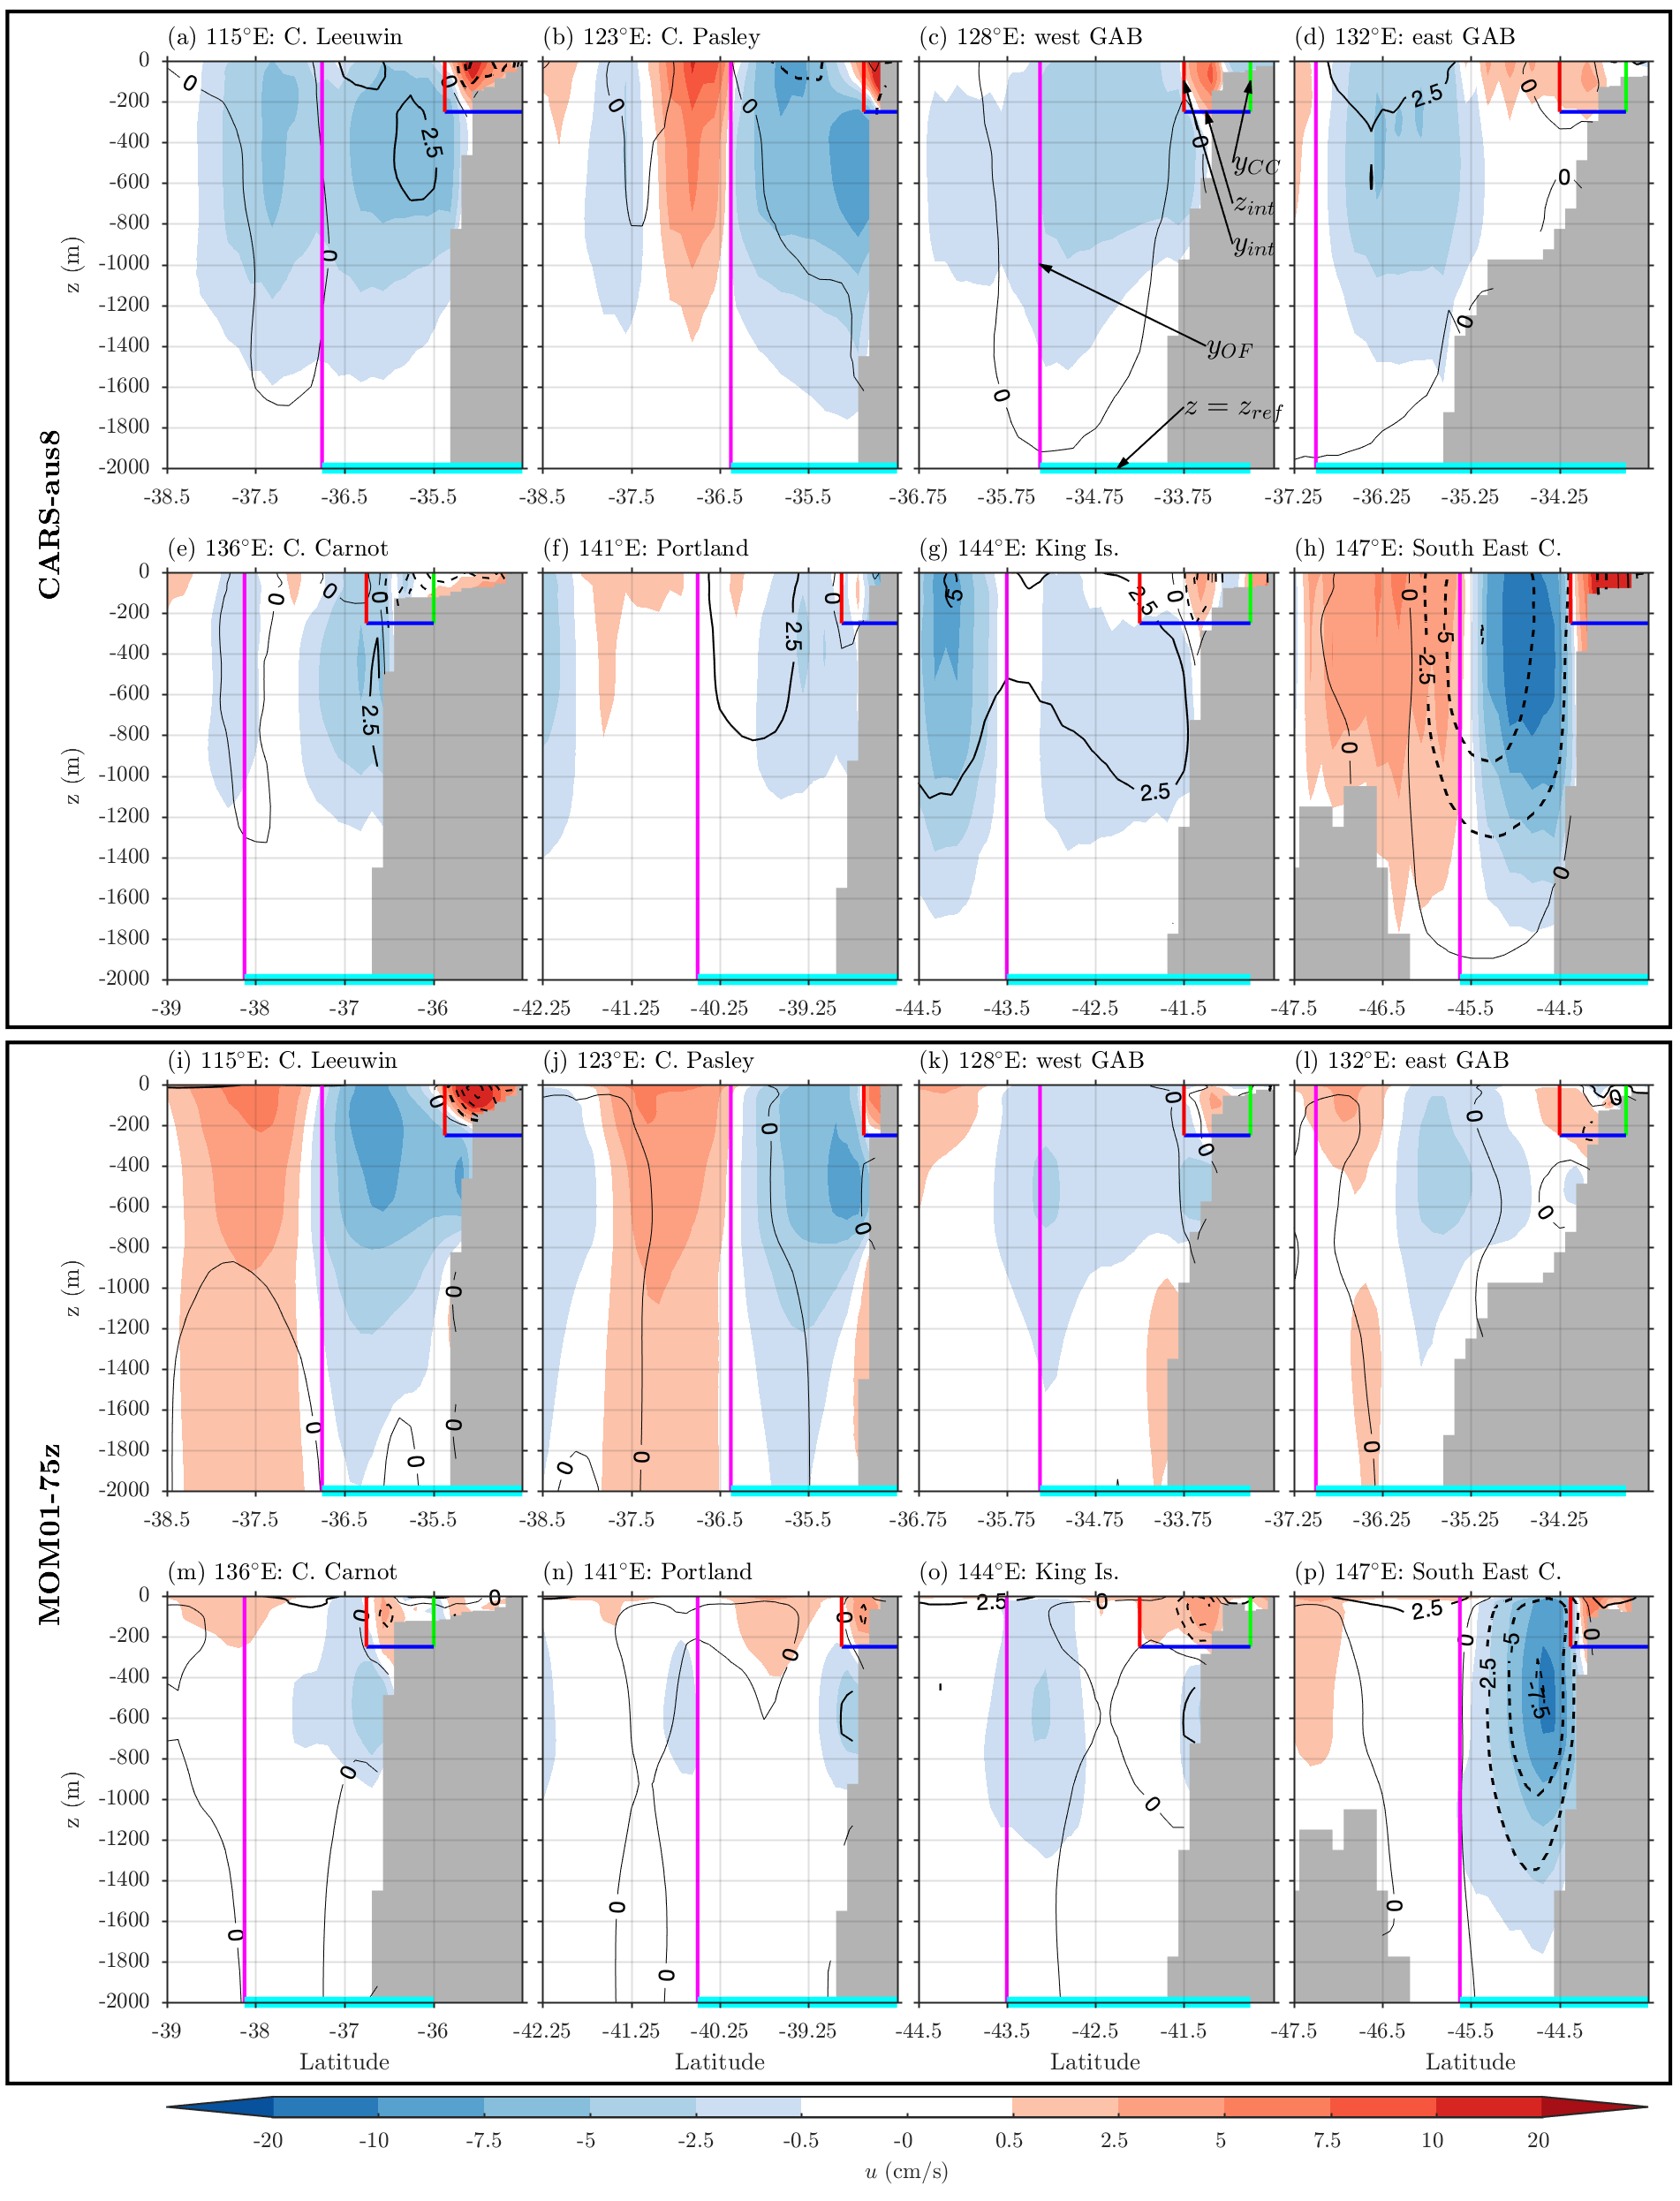
\includegraphics
[width=\textwidth, height=0.89\textheight, keepaspectratio]
{f02_fig1_.png}
\caption{\label{f02_fig1_}%
  Meridional sections along southern Australia of (a-h) geostrophic velocities in CARS and (i-p) full velocities in MOM01. Zonal geostrophic velocities $u\sub{g}$ in CARS (full zonal velocities in MOM01) in \si{\centi\meter\per\second} (shadings, non-monotonic scale) and meridional geostrophic velocities $v\sub{g}$ in CARS (full meridional velocities in MOM01) in \si{\centi\meter\per\second} (contours, every \SI{2.5}{\centi\meter\per\second}, thick solid lines show positive values, thick dashed lines show negative values, thin solid lines show zero contour). Boundaries of the SBC and FC as follows: $y\sub{CC}$ (green) is the SBC north boundary; $z\sub{int}$ (blue) is the SBC bottom boundary and the FC top boundary; $y\sub{int}$ (red) is the SBC south boundary and the FC north boundary; $y\sub{OF}$ (magenta) is the FC south boundary; $z\sub{ref}$ (thick cyan) is the FC bottom closed boundary at the reference depth.}
\end{figure}

While the SBC are relatively narrow, thin and well contained along the shelf break, the FC is wider and thicker, with a varying core position. We define here an \enquote{offshore-FC}
south of the SBC, centered at the surface and extending downward to \SI{2000}{\meter} (Fig.\,\ref{f02_fig1_}b,c,d,f,h), and
a \enquote{slope-FC} at sub-surface centered at \SI{600}{\meter} underneath the SBC and adjacent to the slope (Fig.\,\ref{f02_fig1_}b,c,e,g). The slope-FC forms a clearer separate core from the offshore-FC in MOM01 (Fig.\,\ref{f02_fig1_}i-o).
Hence, the SBC and FC volumes can be defined by separating the water column into an upper layer containing the SBC and upper offshore-FC, and a lower layer containing the slope-FC and lower offshore-FC\@. The horizontal interface $z\sub{int}$ between the upper and lower layers is therefore the SBC bottom boundary. We choose $z\sub{int} = \SI{-250}{\meter}$ (Fig.\,\ref{f02_fig1_}, blue line) as this level is generally very close to, or within, the \num{0} to \SI{4}{\centi\meter\per\second} eastward velocity range at the SBC base. $\Vec{V\sub{up}}$ (Fig.\,\ref{f03_fig1_}a) is the integral of geostrophic velocities from the surface to $z\sub{int}$ plus Ekman drift and $\Vec{V\sub{low}}$ (Fig.\,\ref{f03_fig1_}b) is the integral of geostrophic velocities from $z\sub{int}$ to $z\sub{ref}$; hence

\begin{equation} \label{eq:1}
\Vec{V\sub{up}}(x,y) = \int_{z\sub{int}}^{0}\Vec{v\sub{g}}\ dz + \Vec{V\sub{ek}}
\end{equation}
%
\begin{equation} \label{eq:2}
\Vec{V\sub{low}}(x,y) = \int_{z\sub{ref}}^{z\sub{int}}\Vec{v\sub{g}}\ dz.
\end{equation}
%
These depth integrated velocity fields produce transports per unit width in \si{\square\meter\per\second}. Note that $\Vec{V\sub{up}}$ and $\Vec{V\sub{low}}$ from MOM01 are shown in Fig.\,\ref{f03_fig1_}c,d. In this case we simply used full model velocity integrated in the upper and lower layers, rather than the sum of geostrophic and Ekman velocities. In MOM01, the full model velocities in the SBC and FC are generally stronger than the sum of geostrophic and Ekman velocities (not shown). Therefore the MOM01 full SBC and FC transport will be stronger than MOM01 geostrophic transport (see Section\,\ref{Southern Australia Current System Transport Budget}).
%
\begin{figure}[p]
\centering
\includegraphics%
[width=\textwidth, height=0.92\textheight, keepaspectratio]
{f03_fig1_.png}
\caption{\label{f03_fig1_}%
  Depth integrated (a,b) geostrophic velocities in CARS and (c,d) full velocities in MOM01, showing the velocity field (directional plot) and the zonal component (shadings, non-monotonic scale) in \si{\square\meter\per\second} (ie. transport per unit width). The fields are integrated from (a,c) the surface to \SI{-250}{\meter} and from (b,d) \SI{-250}{\meter} to \SI{-2000}{\meter}. In CARS, (a) shows the sum of geostrophic velocities and Ekman velocities and (b) shows geostrophic velocities only. Boundaries of the SBC and FC as follows: $y\sub{CC}$ (green with black outline) is the SBC north boundary; $y\sub{int}$ (red with black outline) is the SBC south boundary and the FC north boundary; $y\sub{OF}$ (magenta with black outline) is the FC south boundary; $z\sub{int}$ area is the surface bounded by $y\sub{int}$ at south and the slope at north.}
\end{figure}

We present in Fig.\,\ref{Diagram_V3} a Southern Australia Current System three-dimensional schematic diagram to understand transport budget exchanges. This schematic illustrates the SBC eastward transport ($U_{SBC}$ thick light blue arrow) and FC westward transport ($U_{FC}$ thick light yellow arrows), which includes the slope-FC below the SBC, and the offshore-FC upper and lower parts. Inward/outward transports into or out of the SBC or FC are indicated as thin coloured arrows. Here, an increase in SBC transport can be supplied from three sources: southward coastal currents inflows ($V_{CC}$ thin green arrows), northward upper offshore-FC inflows ($V_{SBC}$ thin red arrows), and slope-FC upwelling flows ($W_{SBC}$ thin blue arrows). Similarly, an increase in FC transport can be supplied by three sources: southward SBC inflows into the upper offshore-FC ($V_{FC}$ thin red arrows), SBC downwelling flows into the slope-FC ($W_{FC}$ thin blue arrows), northward ocean interior onshore flows into the offshore-FC ($V_{OF}$ thin magenta arrows).
%
\begin{figure}[hbp]
\centering
\includegraphics%
[width=\textwidth, height=0.89\textheight, keepaspectratio]
{Diagram_V3.pdf}
\caption{\label{Diagram_V3}%
  Southern Australia Current System transport budget schematics. The SBC transport is shown as a thick light blue arrow, the offshore-FC and slope-FC transports as thick light yellow arrows. The shallow coastal currents are shown as a black two-ways arrow. The inward/outward transports into/out of the SBC and FC are shown as thin coloured arrows. The budget includes four transport exchanges: horizontal exchange between coastal currents and SBC (green arrows), horizontal exchange between SBC and upper offshore-FC (red arrows), vertical exchange between SBC and slope-FC (blue arrows) and horizontal exchange between ocean interior onshore flows and offshore-FC (magenta arrows).}
\end{figure}

The SBC and FC control volume boundaries are shown in meridional sections of velocities (Fig.\,\ref{f02_fig1_}) and maps of depth integrated velocities (Fig.\,\ref{f03_fig1_}). Here the boundaries colour match up with transport exchange illustrations in Fig.\,\ref{Diagram_V3}. Note there is no vertical flow across the FC bottom as this boundary is at the reference depth $z\sub{ref}$ (Fig.\,\ref{f02_fig1_}, cyan line). Details of SBC and FC lateral boundaries definition are set out in \ref{SBC and FC lateral boundary definition}.

We note MOM01 shows continuous SBC well incorporated into the SBC control volume (Fig.\,\ref{f03_fig1_}c). Even though CARS is a long-term climatology, it still includes some coastal eddy-like ``noise'' in the region (Fig.\,\ref{f03_fig1_}a), which is likely due to the superposition of eddies recorded at different times. Recently, \citet{Oke2018} found that the Great Australian Bight is rich in mesoscale eddies with surface-intensified currents coherent over the water column. The eddies, which are hypothetically due to the horizontal shear associated with the SBC, are most energetic when the SBC seasonally weaken. In MOM01, the eddies synoptic structure, particularly in the Leeuwin Current Extension region, is evident on transient timescales (not shown). Defining fixed boundaries around the SBC is, however, adequate, because the long-term mean boundary circulation is mostly dominated by geostrophic flows. The SBC's jet like shape is maintained by southward propagating pressure anomalies from the Leeuwin Current System. These pressure anomalies turn eastward along southern Australia \citep{Middleton2007, Ridgway2015}. In winter, the currents are reinforced due to westerly winds intensification and increased onshore Ekman drift \citep{Ridgway2004}. In our fixed boundary SBC definition, any eddies and eddy-like meandering flows crossing a boundary will be captured as an inflow or outflow into the currents. \citet{Furue2017} also applied fixed boundaries for the Leeuwin Current System, because the Leeuwin Current, which co-exists with eddies, is also a jet-like flow.

\subsection{Transport budget derivation} \label{Transport budget derivation}
We calculate the local zonal transport within the SBC and FC volumes,
which we refer to as SBC and FC transport. The in/outward transport across volume boundaries is referred to as cross-boundary transport. As a reminder, in CARS, the SBC transport includes geostrophic flow and Ekman drift. The FC transport includes geostrophic flow and Ekman drift in the upper layer, and geostrophic flow only in the lower layer. In MOM01, we carry out the same calculations and also estimate transports from full velocity.
Below, we provide identities for SBC and FC that connect their transport to cross-boundary transports. The following equations represent a transport in volume per unit time in Sverdrups (\si{Sv},  \SI[parse-numbers=false]{10^6}{\cubic\meter\per\second}).

We choose to use Cartesian coordinates, rather than coast-following, because the currents are narrow and it is difficult to define a coast-following coordinate system that allows mass to be conserved in transport calculations. Our approach ensures mass conservation through careful selection of grid cells in the transport budget, and capturing of all flow into and out of each cell. \ref{Reasoning for defining the SBC transport and the FC transport from their zonal transport} explains our reasoning for choosing Cartesian coordinates over coast-following ones.

We first present the SBC transport and cross-boundary transport equations. The following transport equations are indicated in Fig.\,\ref{Diagram_V3}. The SBC transport $\mathcal{U}\sub{SBC}$ is 

\begin{equation} \label{eq:3}
\mathcal{U}\sub{SBC}(x) = \int_{y\sub{int}(x)}^{y\sub{CC}(x)}{U}\sub{up}\ dy,
\end{equation}
%
where $y\sub{int}$ is the SBC south boundary (Fig.\ref{f03_fig1_}a), $y\sub{CC}$ is the SBC north boundary (Fig.\ref{f03_fig1_}a) and $U\sub{up}$ is the zonal velocity component of (\ref{eq:1}). Hence $\mathcal{U}\sub{SBC}$ represents the upper layer zonal transport bounded by $y\sub{int}$ and $y\sub{CC}$, where positive means an eastward SBC transport. 

The cross-boundary transport from coastal currents and from the offshore-FC into the SBC are 

\begin{equation} \label{eq:4}
\mathcal{V}\sub{CC}(x) = \int_{x\sub{west}}^{x}\Vec{n}\sub{CC}\cdot\Vec{V}\sub{up}\ dl\sub{CC},
\end{equation}
%
\begin{equation} \label{eq:5}
\mathcal{V}\sub{SBC}(x) = \int_{x\sub{west}}^{x}\Vec{n}\sub{int}\cdot\Vec{V}\sub{up}\ dl\sub{int},
\end{equation}
%
where $x\sub{west}$ = \ang{115}E is the SBC western edge longitude, $dl\sub{CC}$ and $dl\sub{int}$ are the line elements of the curves $y\sub{CC}$ and $y\sub{int}$, respectively, from $x\sub{west}$ to $x$, and $\Vec{n}$ is a unit vector perpendicular to $dl$ and pointing into the SBC\@.
$\mathcal{V}\sub{CC}$ and $\mathcal{V}\sub{SBC}$ hence represent the horizontal cross-boundary transport, accumulated from $x\sub{west}$ to $x$, across $y\sub{CC}$ (from coastal currents into the SBC) and $y\sub{int}$ (from offshore-FC into the SBC), respectively. Here, since the transport is accumulated from west to east, positive means a net inflow into the SBC.

The cross-boundary transport from the slope-FC into the SBC is defined as

\begin{equation} \label{eq:6}
\mathcal{W}\sub{SBC}(x)
= \int_{x\sub{west}}^{x} \int_{y\sub{int}(x)}^{y\sub{CC}(x)} \nabla\cdot\Vec{V}\sub{up}\ dy\ dx.
\end{equation}
%
where $y\sub{int}$ is the SBC bottom boundary (Fig.\ref{f02_fig1_}c). Hence $\mathcal{W}\sub{SBC}$ represents the vertical cross-boundary transport, accumulated from $x\sub{west}$ to $x$, across $z\sub{int}$ (from the slope-FC into the SBC). In this accumulated transport, positive means a net upwelling flow into the SBC.

We now describe the FC transport and cross-boundary transport equations. The FC transport $\mathcal{U}\sub{FC}$ is 

\begin{equation} \label{eq:7}
\mathcal{U}\sub{FC}(x) = \int_{y\sub{OF}(x)}^{y\sub{int}(x)}{U}\sub{up}\ dy
+ \int_{y\sub{OF}(x)}^{y\sub{slope}(x)}{U}\sub{low}\ dy,
\end{equation}
%
where $y\sub{OF}$ is the FC south boundary (Fig.\ref{f03_fig1_}a), $y\sub{slope}$ is the slope (north) boundary at $z\sub{int}$, and $U\sub{low}$ is the zonal velocity component of (\ref{eq:2}). Hence $\mathcal{U}\sub{FC}$ represents the zonal transport bounded by $y\sub{OF}$ and $y\sub{int}$ in the upper layer (i.e. the near-surface offshore-FC) and by $y\sub{OF}$ and the slope in the lower layer (i.e. the slope-FC and the deep offshore-FC); where positive means an eastward FC transport.

The cross-boundary transport from South Australian Basin onshore flows, representing inputs from the ocean interior, is defined as

\begin{equation} \label{eq:8}
\mathcal{V}\sub{OF}(x) = \int_{x}^{x\sub{east}}\Vec{n}\sub{OF}\cdot(\Vec{V}\sub{up} + \Vec{V}\sub{low})\ dl\sub{OF},
\end{equation}
%
where $x\sub{east}$ = \ang{147} is the FC eastern edge longitude, $dl\sub{OF}$ is the line element of $y\sub{OF}$ from $x$ to $x\sub{east}$ and $\Vec{n}$ is a unit vector perpendicular to $dl$ and pointing into the FC\@. $\mathcal{V}\sub{OF}$ thus represents the horizontal cross-boundary transport, accumulated from $x$ to $x\sub{east}$, across $y\sub{OF}$ into the FC. Since this transport is accumulated from west to east, positive is a net input from onshore flows into the FC.

The other cross-boundary transports into the FC across $y\sub{int}$ and $z\sub{int}$ are equal and opposite to the corresponding SBC cross-boundary transports (ie. $\mathcal{V}\sub{SBC}$ and $\mathcal{W}\sub{SBC}$, respectively). Hence

\begin{equation} \label{eq:9}
\mathcal{V}\sub{FC}(x) = \int_{x}^{x\sub{east}}-\Vec{n}\sub{int}\cdot\Vec{V}\sub{up}\ dl\sub{int},
\end{equation}
%
\begin{equation} \label{eq:10}
\mathcal{W}\sub{FC}(x) = \int_{x}^{x\sub{east}} \int_{y\sub{int}(x)}^{y\sub{CC}(x)} -\nabla\cdot\Vec{V}\sub{up}\ dy\ dx,
\end{equation}
%
where $\mathcal{V}\sub{FC}$ and $\mathcal{W}\sub{FC}$ represent the cross-boundary transports, accumulated from $x$ to $x\sub{east}$, across $y\sub{int}$ (positive is a net horizontal SBC input) and across $z\sub{int}$ (positive is a net downwelling input from the SBC), respectively.

Finally, since the geostrophic and Ekman velocities (readjusted via the Zero-divergence method, \ref{Zero-divergence method}) and MOM01 full velocities are mass conserving, the SBC transport $\mathcal{U}\sub{SBC}$ and FC transport $\mathcal{U}\sub{FC}$ can also be obtained from the Continuity equation by interpreting the cumulative transport terms (i.e. the cross-boundary transports) as sources and sinks. Hence,

\begin{equation} \label{eq:11}
\mathcal{U}\sub{SBC}(x) = \mathcal{U}\sub{SBC}(x\sub{west}) + \mathcal{V}\sub{CC}(x) + \mathcal{V}\sub{SBC}(x) + \mathcal{W}\sub{SBC}(x).
\end{equation}
%
\begin{equation} \label{eq:12}
-\mathcal{U}\sub{FC}(x) = -\mathcal{U}\sub{FC}(x\sub{east}) + \mathcal{V}\sub{FC}(x) + \mathcal{V}\sub{OF}(x) + \mathcal{W}\sub{FC}(x).
\end{equation}
%
Note that in equation \ref{eq:12}, there is a negative sign in front of $\mathcal{U}\sub{FC}(x)$ because the FC transport is westward, that is in the negative direction, therefore its sign is changed so that inputs into the current (i.e. positive cross-boundary cumulative terms) are translated into a stronger FC. We calculate all transport terms using definitions \ref{eq:3}--\ref{eq:10} and verify that the above equalities are satisfied at very high accuracy. This test is shown in \ref{leak-free}.

\section{Results and Discussion} \label{Results and Discussion}
This section is divided into three subsections. Firstly, we describe the Southern Australia Current System annual-mean, three-dimensional structure (Section~\ref{Southern Australia Current System Structure}). Secondly, we analyse the system transport budget (Section~\ref{Southern Australia Current System Transport Budget}). Finally, we discuss the annual-mean SBC--FC coupling and present an overview of the summer and autumn states (Section~\ref{SBC and FC coupling}).

\subsection{Southern Australia Current System Structure} \label{Southern Australia Current System Structure}
To describe the system structure, we identify the main current features in velocity sections (Section~\ref{Shelf meridional sections}) and in depth integrated velocity maps (Section~\ref{Depth-integrated velocity maps}). In these two subsections we provide enhanced confidence in our findings by comparing the observation-based product CARS with the model data from MOM01. Finally, we examine vertical flows over the shelf MOM01 (Section~\ref{Vertical flows in MOM01}).

\subsubsection{Shelf meridional sections}\label{Shelf meridional sections}
From Cape Leeuwin to Pasley (the two westernmost sections, Fig.\,\ref{f02_fig1_}a,b,i,j), the Leeuwin Current Extension weakens in both CARS and MOM01. Estimates from \citet{Cresswell2004} and \citet{Cresswell1993} also show a stronger Leeuwin Current Extension and more intense eddies near Cape Leeuwin. From the west Great Australian Bight through to King Island (the following five sections, Fig.\,\ref{f02_fig1_}c-g,k-o), the South Australian Current and the Zeehan Current are generally weaker in CARS and MOM01. MOM01 helps identify the current structure in some sections where it is not represented in CARS (e.g. Cape Carnot and Portland sections). Not much is know on the South Australian Current, apart that it is weaker than the Leeuwin Current Extension \citep{Middleton2007} and that it is altered by coastal runoff from the Bight \citep{Rochford1986}. Off South East Cape (easternmost section, Fig.\,\ref{f02_fig1_}h,p), the Zeehan Current intensifies in CARS and MOM01, which is consistent with \citet{Oliver2016,Oliver2018b} who found a strong current there continuing over the eastern Tasmanian shelf. Overall, the SBC are strongest at the western and eastern domain ends (Cape Leeuwin and South East Cape) where they reach mean speed up to \SI{20}{\centi\meter\per\second}.

Since the hydrographic observations fed into CARS are spatially and temporally non-uniform (see \citeauthor{Ridgway2002} \citeyear{Ridgway2002} discussion in Section\,\ref{Datasets}), a CARS versus MOM01 comparison is essential to ensure the current structure and speed represented in CARS is robust. Here, the general agreement between CARS and MOM01 suggests that the topography-adapted interpolation method applied in CARS is suitable to analyse narrow boundary currents at high-resolution. This agreement is impressive given that hydrographic observations over the shallow shelf do not include Argo data, which does not sample in coastal waters shallower than \SI{2000}{\meter}. 

We next identify the FC found offshore and underneath the SBC. Offshore South East Cape, we consider the strong, deep-reaching westward flow to be the Tasman Leakage, following \citepos{Speich2002,vanSebille2012,vanSebille2014} description. We discuss the discontinuity between the Tasman Leakage and FC later, when we analyse velocity maps. Here, we analyse the flow distinction between the slope-FC and offshore-FC along the slanted and the zonal shelf.

The slope-FC is located around \SI{600}{\meter} and found in most sections along the slanted shelf (from Cape Carnot to King Island) and the zonal shelf (from Cape Leeuwin to western Bight). The slope-FC also intensifies to the west towards Cape Leeuwin. Generally, the CARS and MOM01 slope-FC agrees well with \citepos{Middleton2007} velocity records (\num{3}--\SI{7}{\centi\meter\per\second}) and depth range estimates (\num{500}--\SI{1000}{\meter}). At the eastern Bight, the only section with a gentle slope, the slope-FC is absent in CARS and weakest in MOM01. This suggests that a zonal shelf and a steep slope may play a role in maintaining a strong slope-FC. 

The offshore-FC also intensifies to the west towards Cape Leeuwin. The offshore-FC is either weaker or detached from the slope-FC where the shelf slant is strong (Portland and King island sections) and where the slope is gentle (eastern Bight section). While the shelf orientation and slope steepness may play a role in maintaining these FC components, the detachment between the slope-FC and the offshore-FC may indicate they are independent features occasionally merging and separating as the topography varies. Overall, the FC is strongest at Cape Pasley and Cape Leeuwin where it reaches mean speed up to \SI{10}{\centi\meter\per\second}, which agrees well with FC speed records from \citet{Cresswell1993}.

One noticeable difference between CARS and MOM01 is at the Cape Leeuwin section. Here, in CARS, the FC weakens and splits producing another westward flow further offshore. In MOM01, this further offshore flow is eastward. 
In the next sub-Section, we identify this vertically coherent eastward jet as the southern arm of the anti-cyclonic Albany High (\citeauthor{Middleton2003} \citeyear{Middleton2003}, \citeauthor{Middleton2007} \citeyear{Middleton2007}, \citeauthor{McCartney2007} \citeyear{McCartney2007}) clearly visible off Cape Leeuwin and Pasley in MOM01 (and, off Cape Pasley in CARS too).

\subsubsection{Depth-integrated velocity maps}\label{Depth-integrated velocity maps}
We now examine the upper and lower layer velocity fields in depth-integrated velocity maps (Fig.\,\ref{f03_fig1_}). In CARS, the SBC eastward flow is interrupted by reversals, notably near Albany, between Cape Carnot and Cape Jaffa, and west of Tasmania (Fig.\,\ref{f03_fig1_}a). In addition to CARS caveats described in Section\,\ref{Datasets}, localised SBC reversals there may due to the mean field capturing some of the intense eddy activity over the shelf, which was observed in MOM01 on 5-day average timescales (not shown). Regardless, the SBC magnitude and width agree well between CARS and MOM01. In MOM01, the SBC flow is a narrow, continuous eastward boundary current (Fig.\,\ref{f03_fig1_}c).

The narrow slope-FC is not visible, so we next analyse the offshore-FC wide horizontal structure. Along the slanted shelf and in the upper layer, the FC is weak and locally reversed in CARS and MOM01. In the lower layer, the FC is continuous in CARS (Fig.\,\ref{f03_fig1_}b) and more coherent in MOM01 (Fig.\,\ref{f03_fig1_}d), perhaps because the deep flow is less affected by surface intensified mesoscale structures. Along the zonal shelf, the FC firmly emerges as a wide, westward-intensifying westward flow in both layers.

Further offshore, the long-term average field tends to reveal mesoscale structures in CARS and laminar flows in MOM01\@. For example, in CARS, the eastward jet south of the FC is vertically coherent but horizontally patchy, and absent off Cape Leeuwin, due to the FC offshore spreading found earlier (Fig.\,\ref{f02_fig1_}a). In MOM01, the eastward jet is coherent horizontally and vertically, at least until the Great Australian Bight. At South East Cape, the Tasman Leakage outflows via westward-flowing meandering structures in CARS, whereas it outflows mostly due westward in MOM01. In both layers and datasets, the Tasman Leakage flows away from the western Tasmanian shelf and whether some flow is carried into the FC is unclear from these velocity fields. The transport budget in Section\,\ref{Southern Australia Current System Transport Budget} provides insights into the Tasman Leakage-to-FC connection.

\subsubsection{Vertical flows in MOM01} \label{Vertical flows in MOM01}
This section briefly examines vertical flow between the SBC 
and slope-FC\@. Fig.\,\ref{f07_fig1_} shows meridional sections of vertical and zonal components of velocity from MOM01 zoomed in on the shelf break
and the upper slope.
Here, the blue-red shading illustrates vertical flows and the contours show zonal velocities.

Our sections show strong downwelling flows
near the shelf break and upper slope.
These flows are located approximately
on the seaward side and lower portion of the SBC\@.
They are strong between \num{100} and \SI{600}{\meter} and generally intrude into most of the slope-FC, which is centered between \num{500} and \SI{600}{\meter} (Fig.\,\ref{f07_fig1_}a,e,f,g). The Leeuwin Current Extension exhibits a strong downwelling into the slope-FC at Cape Leeuwin (Fig.\,\ref{f07_fig1_}a) with speeds greater than \SI{-50 e-4}{\centi\meter\per\second}.
In the Great Australian Bight sections, the downwelling decreases. In the eastern Bight section (Fig.\,\ref{f07_fig1_}d), where the upper slope is gentle and the slope-FC is absent, an upwelling flow dominates at the South Australian Current bottom boundary. In the subsequent slanted shelf sections at Cape Carnot, Portland and King island (Fig.\,\ref{f07_fig1_}e,f,g) the downwelling is greater than \SI{-20 e-4}{\centi\meter\per\second} and generally stronger than that along the zonal shelf sections (Fig.\,\ref{f07_fig1_}b,c,d, Cape Leeuwin section excluded). Off South East Cape (Fig.\,\ref{f07_fig1_}h), the downwelling dominates the upper \SI{1000}{\meter} and flows through the onshore portion of the Tasman Leakage.
%
\begin{figure}[p]
\centering%
\includegraphics%
[width=\textwidth, height=0.89\textheight, keepaspectratio]%
{f07_fig1_.png}
\caption{\label{f07_fig1_}%
  Meridional sections along southern Australia of vertical and zonal full velocities in MOM01, zoomed over the shelf break region. Vertical velocities $w$ in $10^{-4}$ \si{\centi\meter\per\second} (shadings) and zonal velocities $u$ in \si{\centi\meter\per\second} (contours, every \SI{2}{\centi\meter\per\second}, thick solid lines show positive values, thick dashed lines show negative values, thin solid lines show zero contour). Boundaries of the SBC as follows: $y\sub{CC}$ (green) is the SBC north boundary; $z\sub{int}$ (blue) is the SBC bottom boundary and the FC top boundary; $y\sub{int}$ (red) is the SBC south boundary and the FC north boundary.}
\end{figure}

The slope-FC co-exists with the SBC downwelling coming from above. At the only section where the slope-FC is absent (off the eastern Great Australian Bight Fig.\,\ref{f07_fig1_}d), the vertical flow is upwelling.
This suggests that downwelling is important to maintain the slope-FC\@.
%
Within the lower portion of the FC, a deep upwelling generally exists along the zonal shelf sections and at Cape Carnot (Fig.\,\ref{f07_fig1_}a--e).
In the remaining slanted sections, a weak upwelling exists deeper than \SI{1000}{\meter} (not shown) while
the layer above it is dominated by SBC downwelling.
%
This configuration consisting of a downwelling shelf break current and an upwelling counter-flowing undercurrent (slope current) was also described in \citepos{Woo2008} analysis of the Leeuwin Current System along western Australia who also conjectured that the SBC--slope-FC pair essentially has the same structure as the Leeuwin Current--Leeuwin Undercurrent pair.

To summarise, downwelling flows exist in the lower and seaward portion of the SBC and intrude into the slope-FC\@.
The downwelling flows cover most of the slope-FC, but 
in one section off the eastern Great Australian Bight section, the slope is gentler, the slope-FC is absent, and the vertical flows at the SBC bottom are upwelling. This suggests that both the downwelling and the slope-FC exist where the continental slope is steep. The downwelling is strong at Cape Leeuwin (greater than \SI{-50 e-4}{\centi\meter\per\second}) and extends deeper off the slanted shelf sections (speed greater than \SI{-20 e-4}{\centi\meter\per\second}) and off South East Cape where they dominate the upper \SI{1000}{\meter}. 

\subsection{Southern Australia Current System Transport Budget} \label{Southern Australia Current System Transport Budget}
The CARS and MOM01 long-term mean transport budget (Fig.\,\ref{f04_fig1_}) as derived from the equations in Section~\ref{Transport budget derivation} is analysed for the SBC (Section~\ref{SBC budget}) and the FC (Section~\ref{FC budget}). This budget describes the evolution of the transports for the SBC ($\mathcal{U}\sub{SBC}$, Eq.\,\ref{eq:3}) and the FC ($\mathcal{U}\sub{FC}$, Eq.\,\ref{eq:7});
it also describes
horizontal and vertical inflows into or outflows out of
the SBC which are referenced in Fig.\,\ref{f04_fig1_} ($\mathcal{V}\sub{CC}$, Eq.\,\ref{eq:4}; $\mathcal{V}\sub{SBC}$, Eq.\,\ref{eq:5}; $\mathcal{W}\sub{SBC}$, Eq.\,\ref{eq:6}) and
the FC ($\mathcal{V}\sub{OF}$, Eq.\,\ref{eq:8}; $\mathcal{V}\sub{FC}$, Eq.\,\ref{eq:9}; $\mathcal{W}\sub{FC}$, Eq.\,\ref{eq:10}).
We recall that the sign convention for the zonal transports (Eq.\,\ref{eq:3} and \ref{eq:7}) is that positive means an eastward current. For the cumulative, cross-boundary transports in the horizontal and vertical directions (Eqs.\,\ref{eq:4}, \ref{eq:5}, \ref{eq:6}, \ref{eq:8}, \ref{eq:9} and \ref{eq:10}), positive means into the boundary current and negative means out of the boundary current. Fig.\,\ref{SACS_complex} summarizes the structure of the Southern Australia Current System in detail from both CARS and MOM01. The transport numbers for the model are from the MOM01 full velocity field. This analysis is further summarised and simplified in Section~\ref{Summary} and Fig.\,\ref{Slide1}.

\subsubsection{SBC budget}\label{SBC budget}
The SBC transport $\mathcal{U}\sub{SBC}$ (Eq.\,\ref{eq:3}, Fig.\,\ref{f04_fig1_}a black lines) exhibits significantly higher variations in CARS than in MOM01, particularly in the Leeuwin Current Extension (see also Fig.\,\ref{f03_fig1_}).
High variations are probably due to the mean CARS data being locally biased towards particular transient, seasonal or inter-annual events. Nonetheless, the trend of the South Australian Current and the Zeehan Current transport in CARS
roughly agrees with those in MOM01. It is worth noting here that in MOM01, the transport adjusted via the Zero Divergence method (i.e., Ekman plus geostrophic transport from the Zero Divergence method applied to the model's temperature and salinity field and wind data) agrees very well with the full transport determined from the model's full velocity field. In the full MOM01 transport, the Leeuwin Current Extension decreases from $\mathcal{U}\sub{SBC} =$ \num{1.1} to about \SI{0.1}{Sv}, the South Australian Current fluctuates with the transport across the zonal shelf remaining stable and that across the the slanted shelf increasing to \SI{0.3}{Sv}, and the Zeehan Current slightly increasing to about \SI{0.4}{Sv} (Fig.\,\ref{SACS_complex}).
%
\begin{figure}[p]
\noindent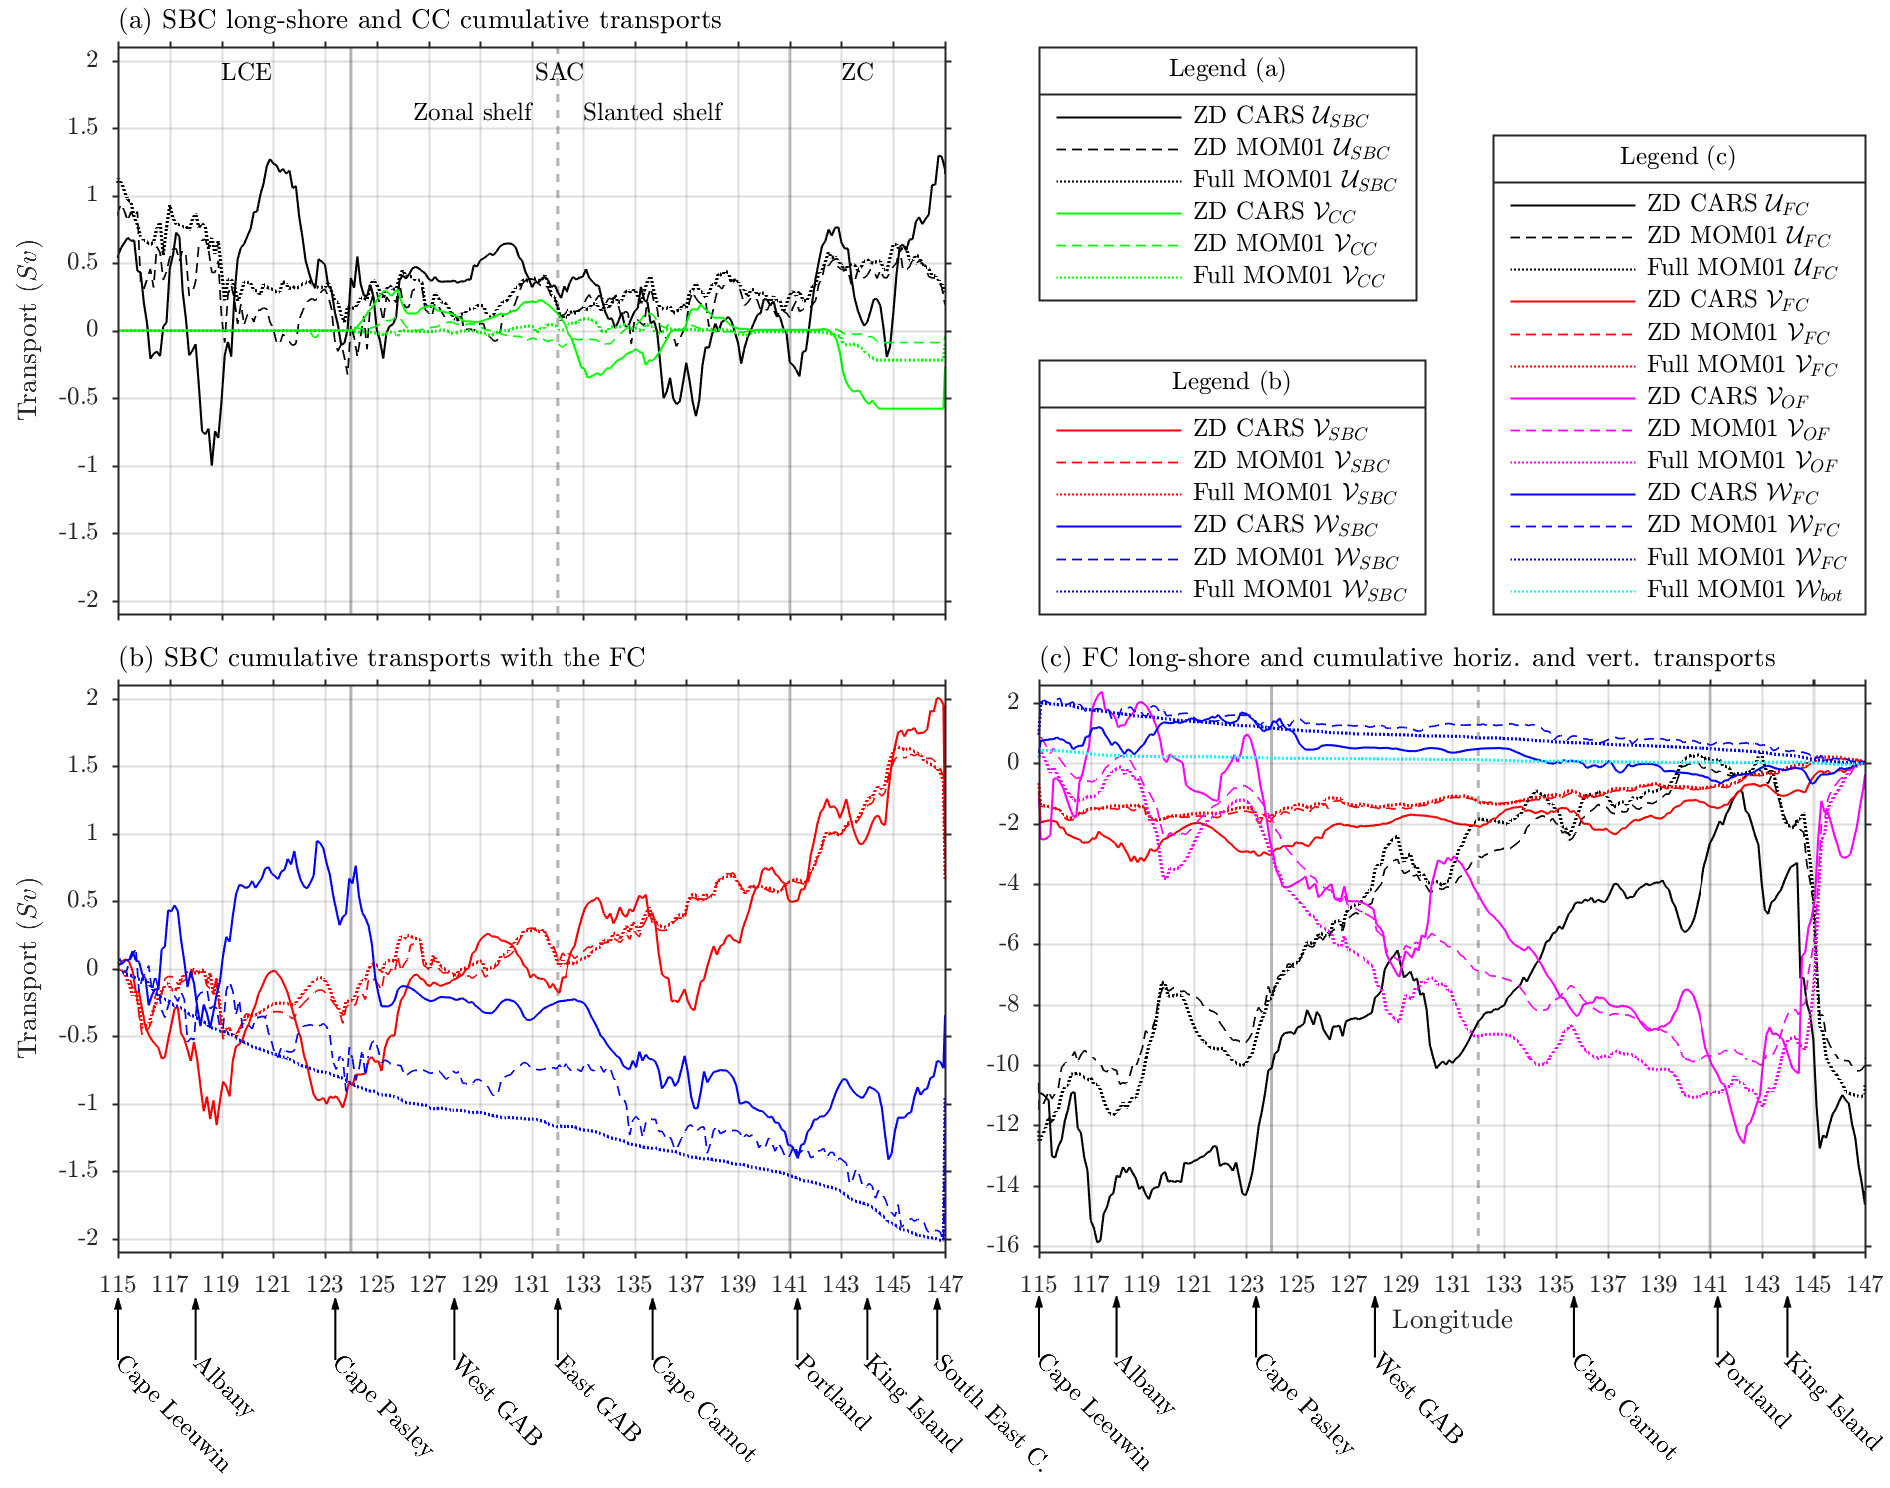
\includegraphics
[width=\textwidth, height=0.89\textheight, keepaspectratio]
{f04_fig1_.png}
\caption{\label{f04_fig1_}%
  Southern Australia Current System transport budget ($Sv$) for (a) the SBC transport (black, positive eastward) and the horizontal cumulative (west to east) cross-boundary transport along $y\sub{CC}$ (green, positive into the SBC), (b) the SBC cumulative (west to east) cross-boundary transport exchanged with the FC horizontally across $y\sub{int}$ (red, positive into the SBC) and vertically across $z\sub{int}$ (blue, positive into the SBC), (c) the FC transport (black, positive eastward), cumulative (east to west) cross-boundary transports with the SBC (red and blue, positive into the FC), and cumulative (east to west) cross-boundary horizontal transport along $y\sub{OF}$ (magenta, positive into the FC). Results are shown for the "Zero Divergence" (ZD, \citeauthor{Furue2017} \citeyear{Furue2017}) adjusted transports in the observations (solid lines) and in the model (dashed lines), and also the actual model transports (thin dotted line). The thin dotted cyan line shows the actual model vertical transport at the bottom of the FC (this is absent in the geostrophic transport). The vertical solid gray lines separate the Leeuwin Current Extension, South Australian Current and Zeehan Current and the vertical dashed grey line separates the region with a zonal shelf to the west from the region with a slanted shelf to the east.}
\end{figure}
%
\begin{figure}[p]
\noindent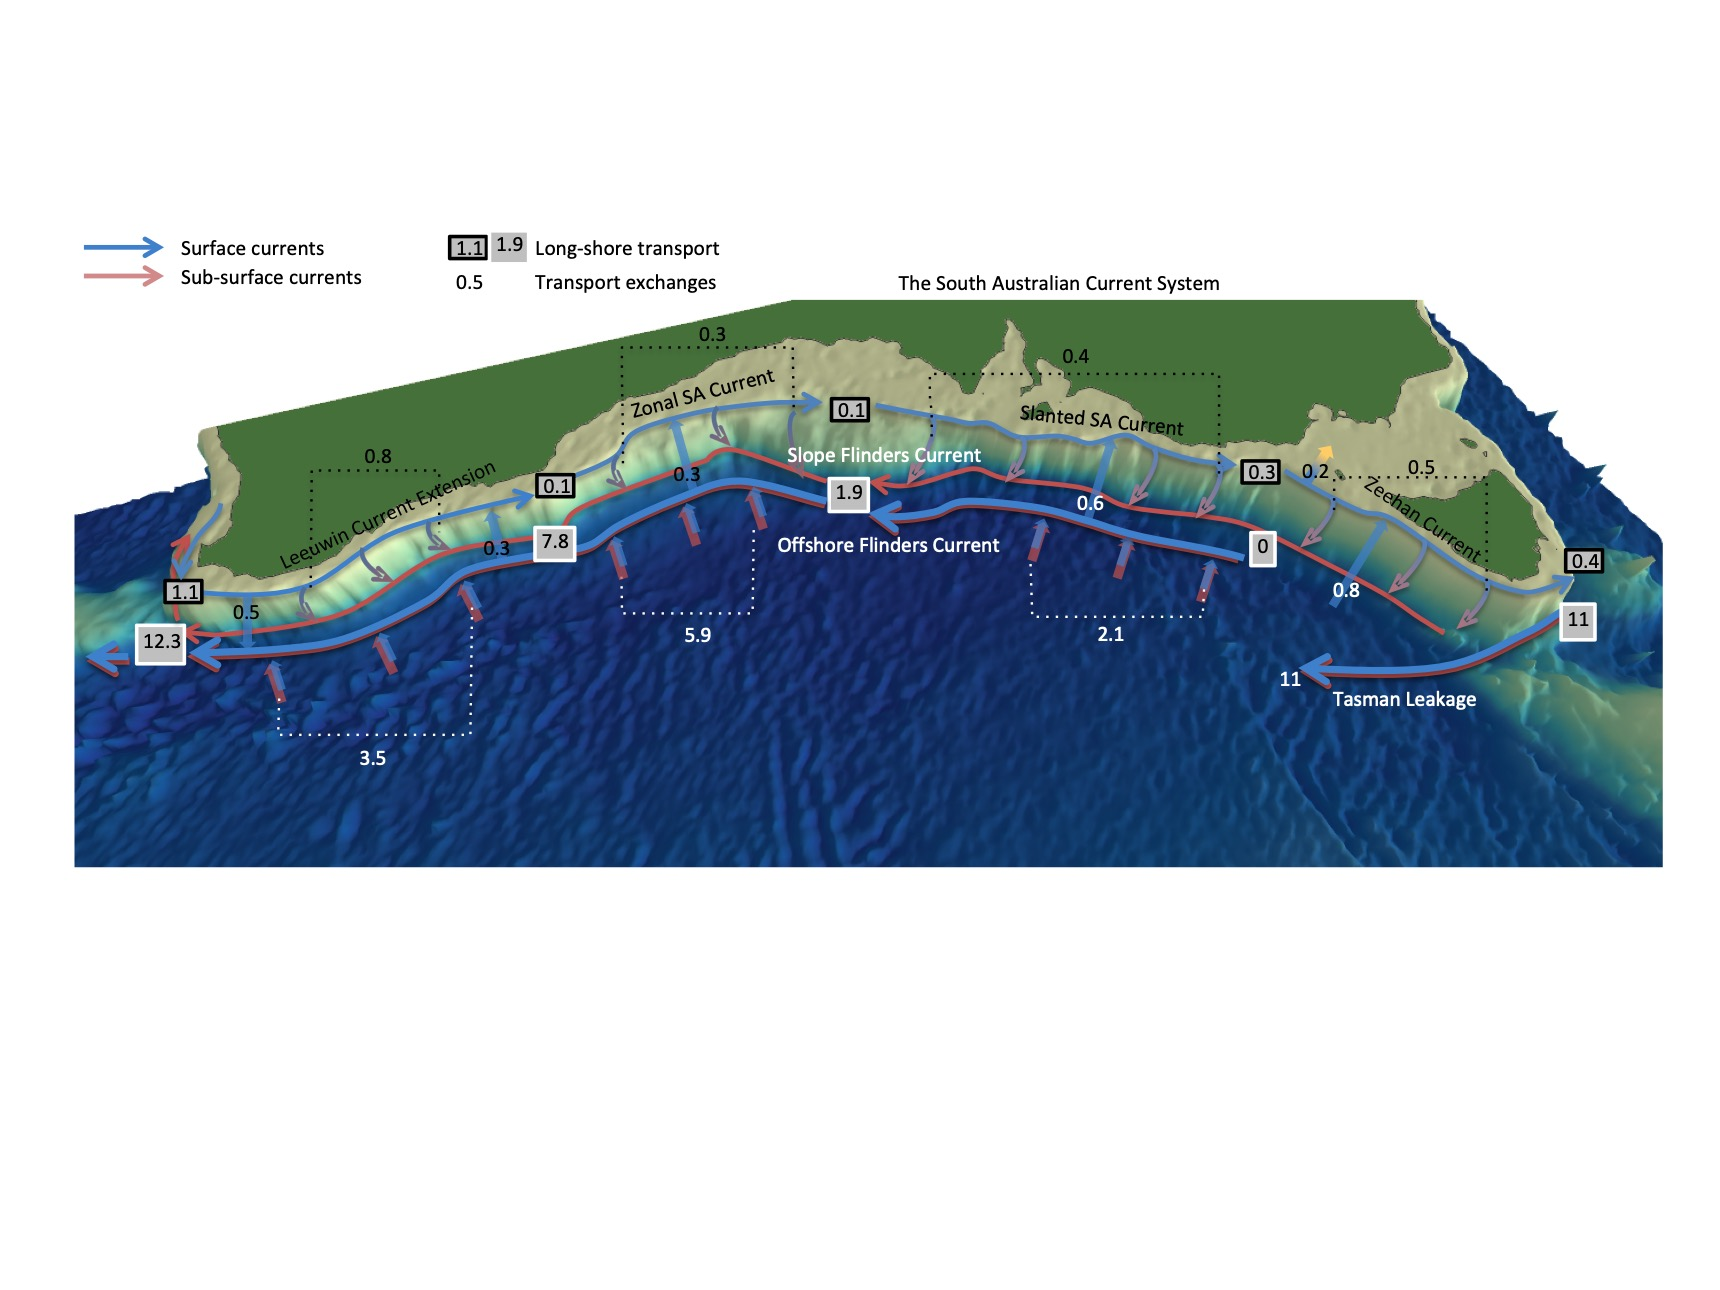
\includegraphics
[width=1\textheight, height=\textwidth, keepaspectratio, angle=90]
{SACS_complex.jpg}
\caption{\label{SACS_complex}%
  Comprehensive Southern Australia Current System transport budget schematics ($Sv$). Transport estimates from MOM01 reported in Section~\ref{Southern Australia Current System Transport Budget} are illustrated here. The SBC transport $\mathcal{U}\sub{SBC}$ (Eq.\,\ref{eq:3}) is shown in the grey box with a black outline. The FC transport $\mathcal{U}\sub{FC}$ (Eq.\,\ref{eq:7}) is shown in the grey box with a white outline. The transport exchanges feeding into the SBC or the FC are shown as plain white or black numbers.}
\end{figure}

The cumulative cross-boundary transport between the coastal current and SBC $\mathcal{V}\sub{CC}$ (Eq.\,\ref{eq:4}, Fig.\,\ref{f04_fig1_}a green lines) in CARS generally exhibits a net inflow into the SBC along the zonal shelf west of \ang{132}E and a net outflow from the SBC along the slanted shelf east of \ang{132}E. These exchanges in the Great Australian Bight and Gulf regions are much weaker in MOM01 with a weak net inflow up to $\mathcal{V}\sub{CC} =$ +\SI{0.1}{Sv}. Since the Bight and Gulfs region
is land-locked, this net transport returns to zero at Cape Jaffa (\ang{139}E)
 and hence this pair of inflow and outflow represents a mean counter-clockwise circulation over the shelf within the Bight and Gulfs.
Over Bass Strait,
there is a net outflow from the SBC of \SI{0.2}{Sv} (Fig.\,\ref{SACS_complex}) in MOM01,
which is half that in CARS\@.

The cumulative cross-boundary transport between the SBC and the FC are presented in Fig.\,\ref{f04_fig1_}b. As seen in the SBC transport, the Leeuwin Current Extension is a region of large difference
between CARS and MOM01,
which is reflected in both the horizontal exchanges with the FC along the SBC south boundary $\mathcal{V}\sub{SBC}$ (Eq.\,\ref{eq:5}, Fig.\,\ref{f04_fig1_}b red lines) and the vertical exchanges with the FC along the SBC bottom boundary $\mathcal{W}\sub{SBC}$ (Eq.\,\ref{eq:6}, Fig.\,\ref{f04_fig1_}b blue lines).
Further east, the downstream trends in the horizontal and vertical exchanges agree reasonably well between CARS and MOM01.
In MOM01, on average the Leeuwin Current Extension loses water horizontally to the FC as the cumulative horizontal transport is negative in the entire Leeuwin Current Extension region. Specifically, the Leeuwin Current Extension loses $\mathcal{V}\sub{SBC} = \SI{-0.5}{Sv}$ up to \ang{119}E near Albany (Fig.\,\ref{SACS_complex}), which indicates
that the Leeuwin Current partly outflows horizontally into the offshore-FC as it turns around the south-west corner of Australia to become the Leeuwin Current Extension\@. East of Albany, the opposite happens where the upper offshore-FC generally feeds horizontally into the SBC\@. In Fig.\,\ref{SACS_complex} we report the horizontal inflows from the FC into each of the SBC. The total horizontal inflow into the SBC from Cape Leeuwin to South East Cape is +\SI{1.5}{Sv}.

The model vertical exchanges between the SBC and the FC reveal a persistent downwelling out of the SBC that increases steadily from west to east \@. To this downwelling, the Leeuwin Current Extension contributes $\mathcal{W}\sub{SBC} =$ \SI{-0.8}{Sv}, the South Australian Current \SI{-0.7}{Sv} and the Zeehan Current \SI{-0.5}{Sv} (Fig.\,\ref{SACS_complex}). This provides a total downwelling of \SI{-2}{Sv} out of the SBC between Cape Leeuwin and South East Cape (Fig.\,\ref{Slide1}).
Eighty percent of the decrease in the Leeuwin Current Extension's transport from
$\mathcal{U}\sub{SBC} = \num{1.1}$ to \SI{0.1}{Sv} is
due to the downwelling.
The zonal South Australian Current's steady transport of \SI{0.1}{Sv} is maintained by compensating lateral inflows that balance the downwelling in this region. The weak increase
in the slanted South Australian Current's transport and the Zeehan Current's transport is essentially due to an increase in lateral inflows.

To summarise, as the Leeuwin Current Extension flows around the southwest corner of Australia, it loses most of its transport due to downwelling
 and lateral offshore flow.
Then the downwelling is reduced and the western South Australian Current flows along the zonal shelf break without much systematic change in its transport.
As the South Australian Current flows over the slanted shelf break, it receives progressively increasing lateral inflows which are partly overturned by weakly increasing downwelling flows, resulting in a stronger slanted South Australian Current\@.
The Zeehan Current grows
in a similar way,
where the lateral inflow is
strong enough to overcome the losses to the downwelling and a lateral outflow into
Bass Strait. Overall, the SBC transport decreases from $\mathcal{U}\sub{SBC} = \SI{1.1}{Sv}$
at Cape Leeuwin to \SI{0.4}{Sv} at South East Cape is due to a $\mathcal{V}\sub{SBC} = +\SI{1.5}{Sv}$ lateral inflow from the FC minus
a $\mathcal{W}\sub{SBC} = \SI{-2}{Sv}$ downwelling 
back into the FC and a weak lateral $\mathcal{V}\sub{CC} = \SI{-0.2}{Sv}$ shallow loss into Bass Strait.

\subsubsection{FC budget}\label{FC budget}
The FC and cross-boundary cumulative transports are presented in Fig.\,\ref{f04_fig1_}c.
The transport $\mathcal{U}\sub{FC}$ (Eq.\,\ref{eq:7}, Fig.\,\ref{f04_fig1_}c black lines) displays large variations in CARS
as for the SBC\@.
Here the FC is generally stronger in CARS than in MOM01, a difference we noted earlier in the velocity maps (Fig.\,\ref{f03_fig1_}), with a westward transport in the observations up to \SI{6}{Sv} stronger.
In CARS, $\mathcal{U}\sub{FC}$ suddenly becomes
weaker between \ang{117} and \ang{116}E
because of the meridional spreading of the FC noted earlier (Fig.\,\ref{f03_fig1_}a,b).
Otherwise the spatial trends between CARS
and MOM01 are similar.
Both in CARS and MOM01,
the transport undergoes
a sudden loss in westward transport
because of the Tasman Leakage
(see also Fig.\,\ref{f03_fig1_}).
In the model, it varies from $\mathcal{U}\sub{FC} = \SI{-11}{Sv}$
at South East Cape to around zero near Portland (a negative transport is westward). The FC then intensifies along the slanted coast to reach \SI{-1.8}{Sv} at the eastern Great Australian Bight; and along the zonal coast to reach \SI{-7.7}{Sv} at Cape Pasley and \SI{-12.3}{Sv} at Cape Leeuwin (Fig.\,\ref{SACS_complex}). In contrast to the SBC,
the FC thus intensifies systematically as it flows westward.

The exchanges between the FC and the SBC are relatively insignificant in determining this increase in the FC transport as the main contributors to the FC strengthening are the
onshore flows
across the FC's southern boundary (Eq.\,\ref{eq:8}).
The spatial structure of the change
in $\mathcal{U}\sub{FC}$ therefore mirrors
that of $\mathcal{V}\sub{OF}$ (Fig.\,\ref{f04_fig1_}c).

Between South East Cape and \ang{143}E, there is a large outflow of \SI{-11}{Sv},
which is the Tasman Leakage.
From South East Cape to Portland (the Zeehan Current region), the Tasman Leakage loss, the exchanges between the SBC and the FC, and small inputs by onshore flows, result in a zero FC transport at Portland.
In what follows, we describe how $\mathcal{U}\sub{FC}$ changes
in relation to $\mathcal{V}\sub{OF}$, ignoring exchanges with the SBC\@.
%
Between Portland and the eastern Great Australian Bight (the slanted South Australian Current region), the onshore flows provide +\SI{2.1}{Sv} to the FC producing a \SI{-1.9}{Sv} FC transport.
Along the zonal coast, between the eastern Bight
and Cape Pasley (the zonal South Australian Current region), the onshore flows provide a large +\SI{5.9}{Sv} input that
accelerates the FC to \SI{-7.8}{Sv}. Finally, between Cape Pasley and Cape Leeuwin (the Leeuwin Current Extension region), the onshore flows provide a +\SI{3.5}{Sv} input further accelerating the FC to \SI{-12.3}{Sv} (Fig.\,\ref{SACS_complex}).

As an aside, we note that we calculated the accumulated vertical transport along the FC's bottom boundary across $z\sub{ref}$ (Fig.\,\ref{f04_fig1_}c cyan lines and Fig.\,\ref{f02_fig1_}i--p cyan lines).
In our geostrophic calculation, vertical velocity is adjusted to vanish at $z\sub{ref}$.
In the actual velocity field of MOM01, there is a total
upward transport across the \SI{2000}{\meter} depth level of about +\SI{0.25}{Sv}
between South East Cape and Cape Leeuwin, which is very small compared to the FC's large westward transport.
This demonstrates that our choice $z\sub{ref} = \SI{2000}{m}$
was suitable.

In summary, the annual-mean FC is nearly absent off the western Tasmanian shelf and Bass Strait as the Tasman Leakage carries
most
of the westward flow off South East Cape into the South Australian Basin. Along the slanted shelf the FC is weak as the onshore flows feeding into the current are small. When the shelf becomes zonal,
the onshore flows are much stronger, providing a large source water for the FC\@.
Overall, after the Tasman Leakage loss (\SI{-11}{Sv}),
the FC transport increases from zero to $\mathcal{U}\sub{FC} = \SI{-12.3}{Sv}$
at Cape Leeuwin due to a net +\SI{11.8}{Sv} gain from the onshore flows (Fig.\,\ref{Slide1}). Out of this net inflow, 2.5\% occurs west of Tasmania, 17.8\% along the slanted shelf, 50\% in the zonal Great Australian Bight region and 29.7\% in the zonal shelf region from Cape Carnot to Cape Leeuwin. Therefore, nearly 80\% of the onshore flow contribution to the FC increase occurs along the zonal shelf. Another \SI{+0.5}{Sv} net gain from the SBC comes from downwelling flows which only contribute to about 4.1\% of the FC's total increase. 

\subsection{SBC and FC coupling}\label{SBC and FC coupling}
The Southern Australian Current System transport budget revealed that a large part of the onshore flow into the FC is directly converted into increasing westward transport from close to zero along western Tasmania to \SI{12.3}{Sv} near the western side of Australia.

Further inshore, there is a coupling between the SBC and offshore-FC which provides a lateral source water for the SBC\@. We examine maps of Ekman drift in Fig.\,\ref{f18_fig1_} to provide a mechanism for such lateral inflow into the SBC\@. We find that the annual-mean Ekman drift in ERA-Interim (which was used with the CARS geostrophic velocities to calculate the transport in CARS, Fig.\,\ref{f18_fig1_}a) is slightly stronger than the Ekman drift in CORE2-NYF (which was used to force MOM01, Fig.\,\ref{f18_fig1_}b). The Ekman drift is generally pointing northward, hence onshore everywhere except in the Great Australian Bight and southeast in front of the Gulfs where it decreases and turns westward. The onshore Ekman drift provides a coupling mechanism between the offshore-FC and SBC, explaining the lateral inflow from the offshore-FC into the SBC.
%
\begin{figure}[htp]
\noindent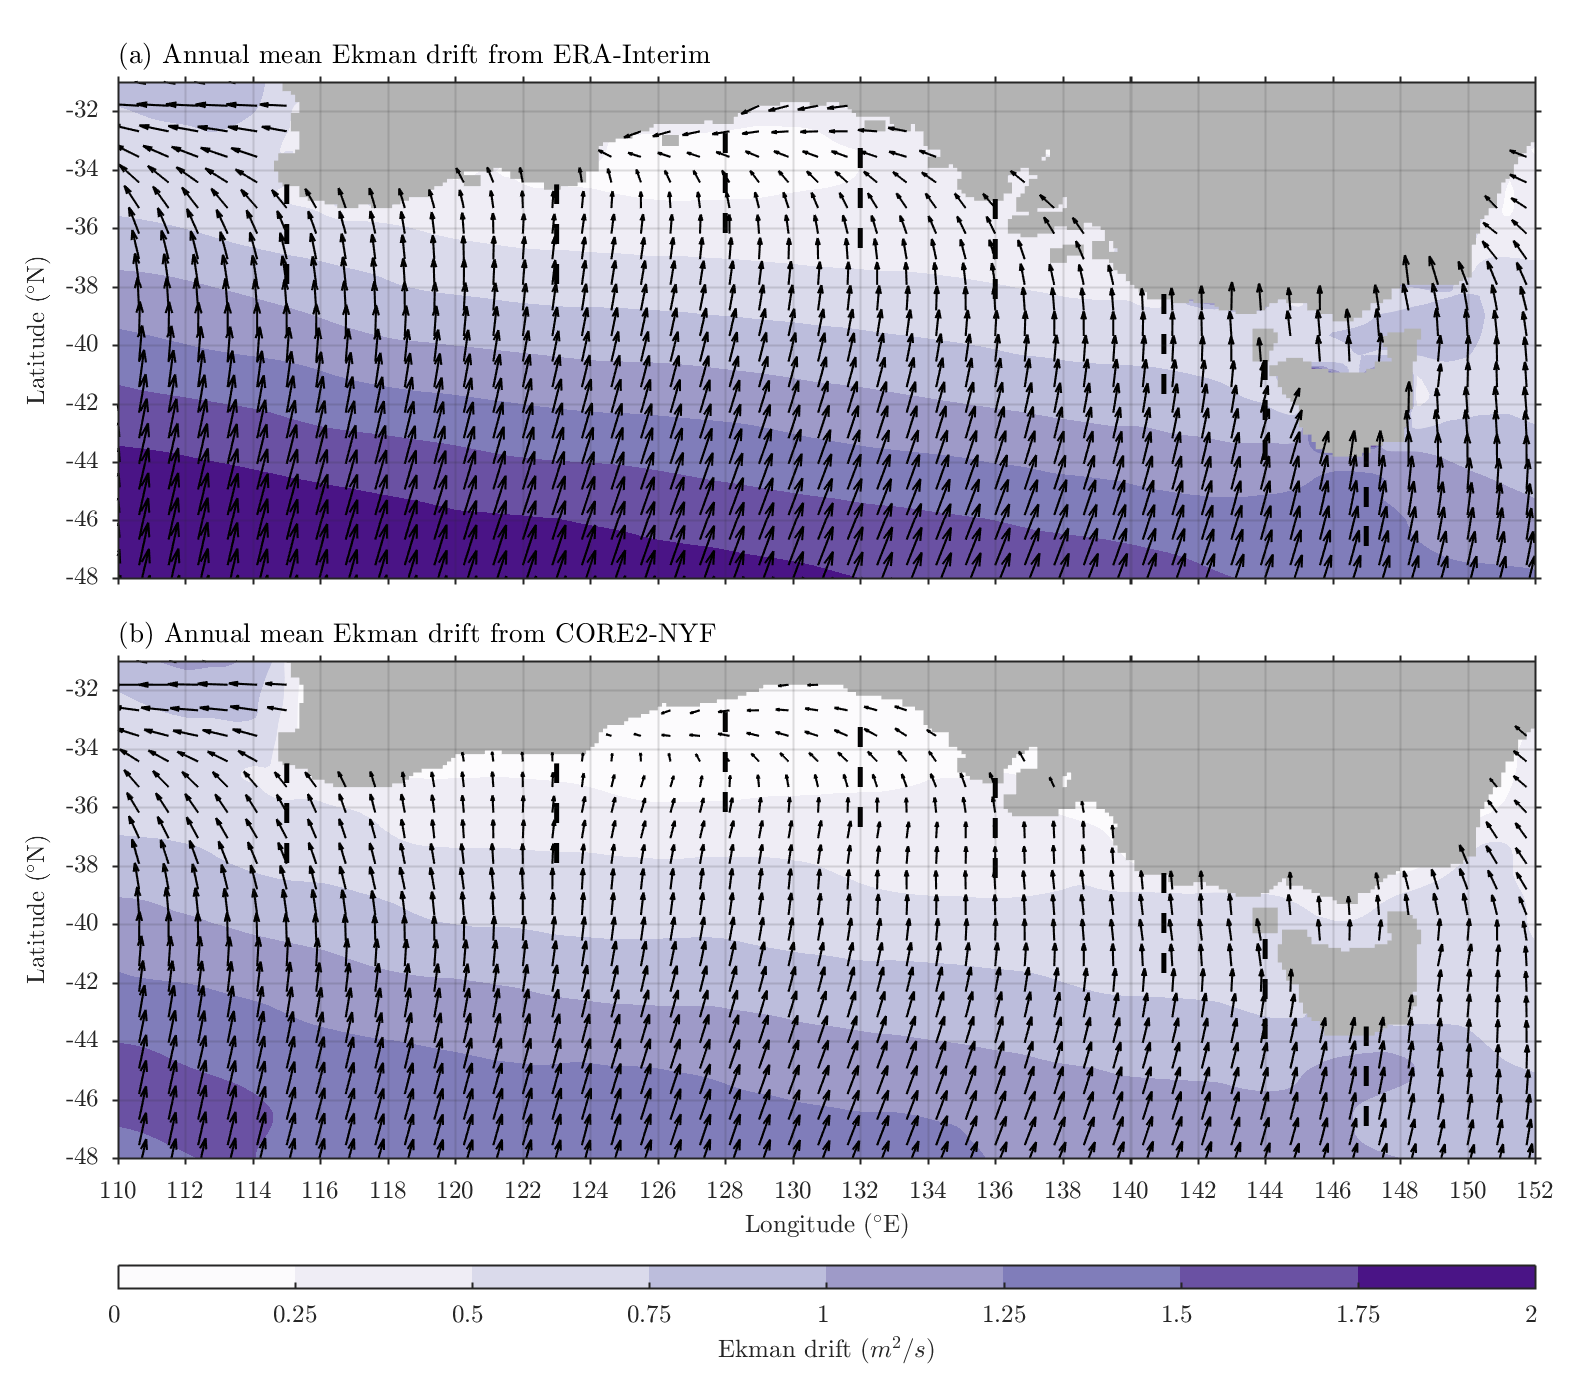
\includegraphics
[width=\textwidth, height=0.89\textheight, keepaspectratio]
{f18_fig1_.png}
\caption{\label{f18_fig1_}%
    Long-term mean Ekman drift (\si{\square\meter\per\second}) estimated from (a) ERA-Interim winds and (b) CORE2-NYF winds (see Section~\ref{Datasets}). The magnitude of the Ekman drift is indicated by the shading. To illustrate weaker flows better, arrow lengths are proportional to the square root of the vector amplitudes.}
\end{figure}

The transport budget also revealed a coupling between the SBC and the slope-FC where the aforementioned Ekman drift is downwelled into the slope-FC\@. We examine maps of vertical flows along $z\sub{int}$ in MOM01 in Fig.\,\ref{f16_fig1_} to examine the spatial variability of the annual-mean downwellings along the coast. We note that we do not show the vertical velocities produced by the Zero-Divergence adjustment, neither in this Figure nor in Fig.\,\ref{f07_fig1_}. This is because the geostrophic calculation (before and after the Zero-Divergence adjustment) produces a noisy vertical-velocity field above complex bottom topography (evident in Fig.\,\ref{f04_fig1_}b,c in local reversal in accumulated upwellings/downwellings). Thus, these fields are useful only when integrated over a long distance as in our cumulative transport calculations. For example, the longshore integration of vertical velocities at the base of the SBC (Eq. \ref{eq:6}) reveals the vertical velocity that compensates the SBC flow above it.
%
\begin{figure}[ht]
\noindent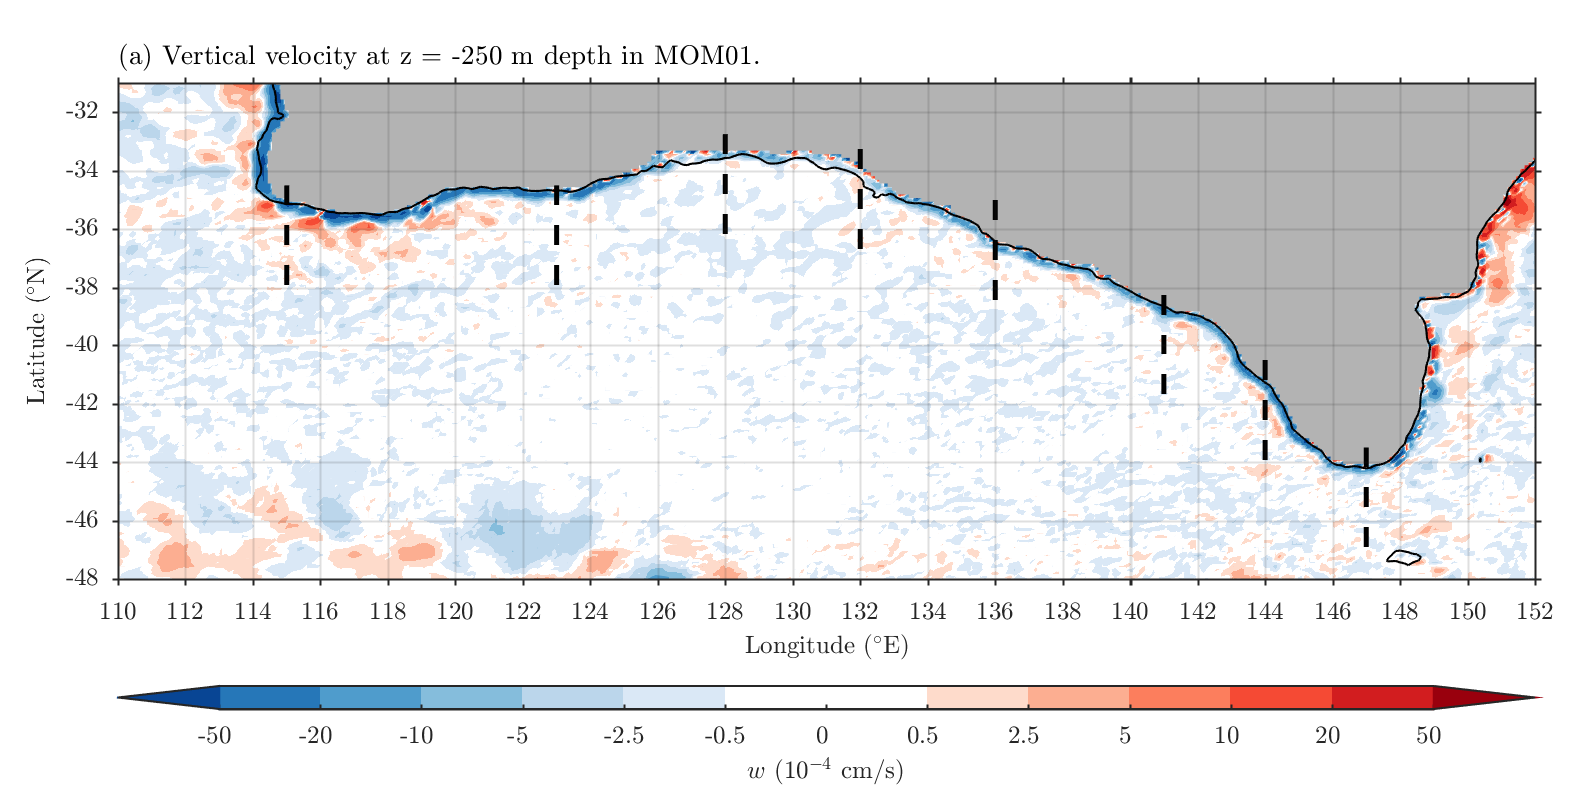
\includegraphics
[width=\textwidth, height=0.89\textheight, keepaspectratio]
{f16_fig1_.png}
\caption{\label{f16_fig1_}%
    Long-term mean full model vertical velocity field at $z\sub{int} = -250$ \si{\meter} in $10^{-4}$ \si{\centi\meter\per\second} (with nonlinear shading levels) in MOM01. The thin black line shows the 1000 \si{\meter} isobath. The grey region is where $z > -250 m$.}
\end{figure}

The vertical flows along the upper slope at \SI{-250}{\meter} are downwelling throughout the southern Australian shelves. The downwelling is strong where the slope is steep particularly outside the Great Australian Bight region. In the Bight, the slope is less steep and the downwelling is weaker. The primarily onshore direction of the Ekman drift is consistent with the downwelling found all along the coast. The downwelling is most pronounced in the Leeuwin Current Extension and Zeehan Current regions, where the onshore Ekman drift is strongest (Fig.\,\ref{f18_fig1_}). In the Bight and Gulf regions the Ekman drift curls anti-clockwise resulting in weak downwelling, which is further reduced in the Bight where the slope is less steep.

Finally, there is also an inverse seasonal relationship between the SBC and the FC which we briefly discuss here. Fig.\,\ref{f19_fig1_} shows the summer and autumn states in MOM01 for the SBC transport ($\mathcal{U}\sub{SBC}$, Fig.\,\ref{f19_fig1_}a) and the FC transport ($\mathcal{U}\sub{FC}$, Fig.\,\ref{f19_fig1_}b). We show the summer and the autumn states only as they exhibit the strongest deviation from the annual-mean. Winter and spring states are much closer to the annual-mean (not shown). \citet{Oke2018} also found that the SBC are strongest in autumn, decrease in winter and spring and are weakest in summer. 
%
\begin{figure}[p]
\noindent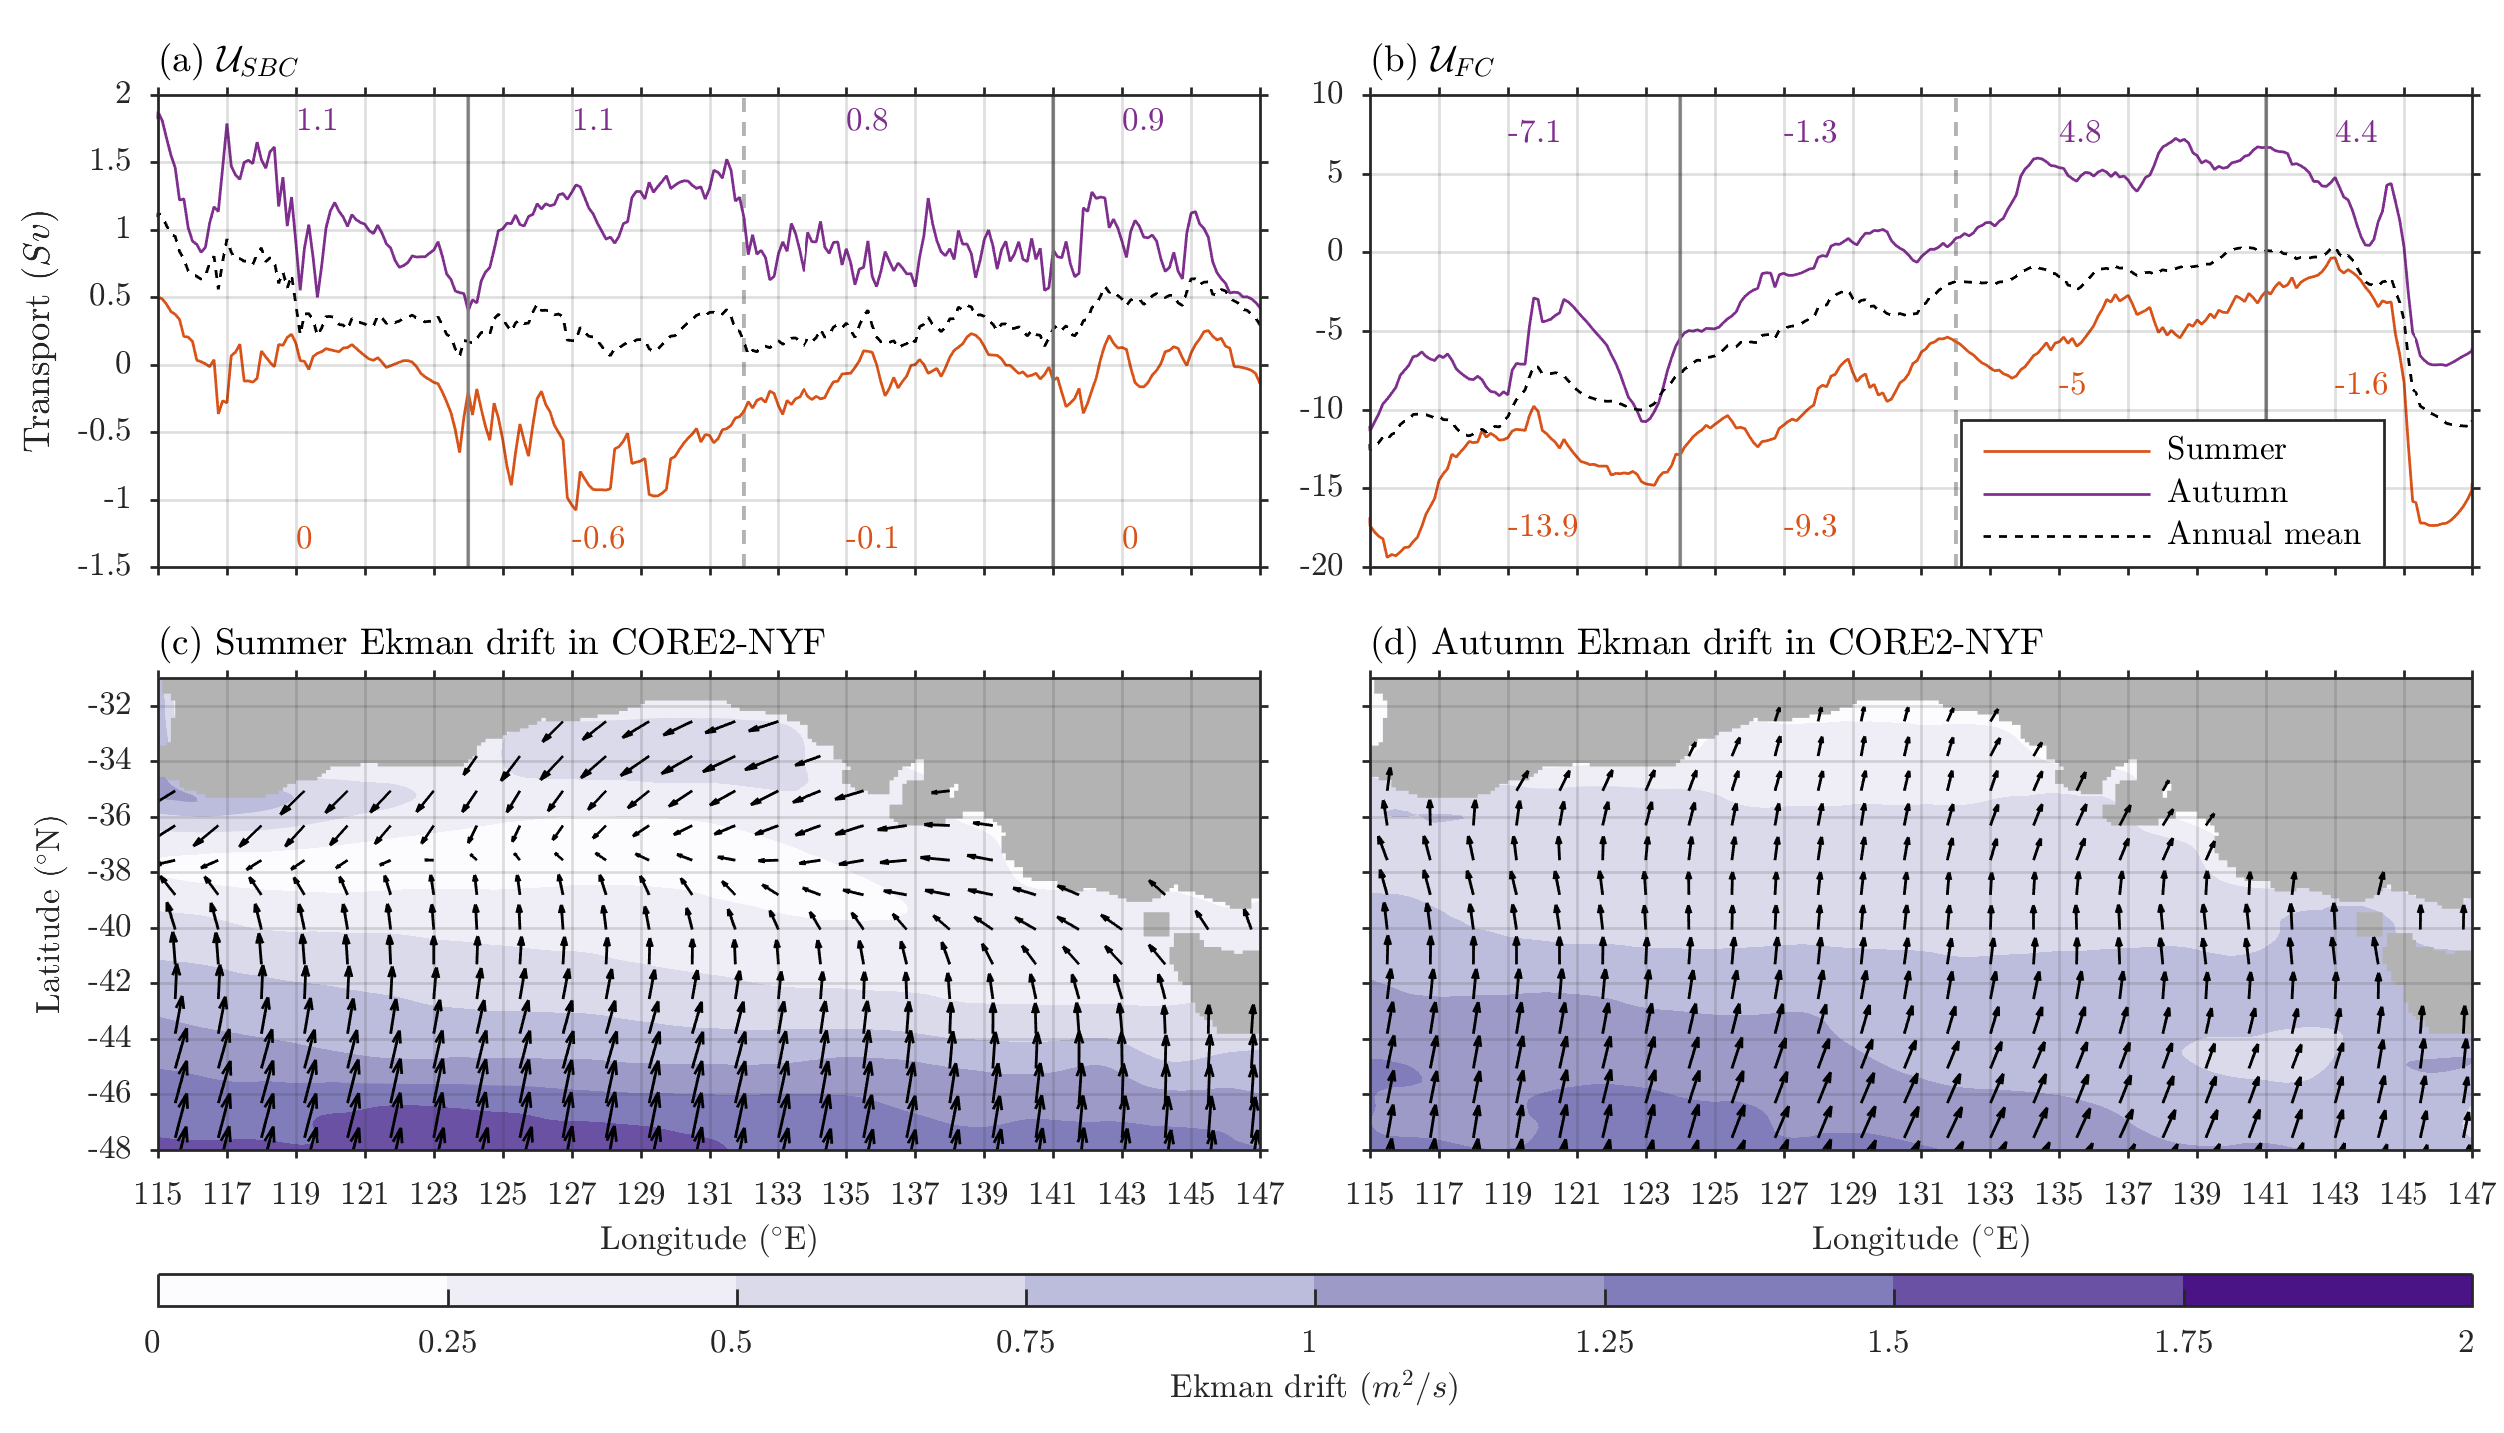
\includegraphics
[width=\textwidth, height=0.89\textheight, keepaspectratio]
{f19_fig1_.png}
\caption{\label{f19_fig1_}%
    Summer mean (orange lines), autumn mean (purple lines), annual-mean (black dashed lines) in MOM01 for (a) the SBC transport ($\mathcal{U}\sub{SBC}$, positive eastward) and (b) the FC transport ($\mathcal{U}\sub{FC}$, positive eastward); and Ekman drift derived from CORE2-NYF winds in (c) summer and (d) autumn. In (a) and (b), the vertical solid gray lines separate the Leeuwin Current Extension, South Australian Current and Zeehan Current and the vertical dashed grey line separates the region with a zonal shelf to the west from the region with a slanted shelf to the east. The coloured numbers in (a) and (b) show, from left to right, the mean transport in the Leeuwin Current Extension region, the zonal South Australian Current region, the slanted South Australian Current region and the Zeehan Current region in summer (orange) and in autumn (purple). In (c) and (d), the magnitude of the Ekman drift is indicated by the shading whereas arrow lengths are proportional to the square root of the vector amplitudes.}
\end{figure}

In summer, the SBC are weakest and reversed in many places along the coast, particularly in the zonal South Australian Current region (Fig.\,\ref{f19_fig1_}a). On average, the Leeuwin Current Extension, the slanted South Australian Current and the Zeehan Current carry very little eastward transport, and the zonal South Australian Current is strongly westward at \SI{0.6}{Sv} on average with a maximum westward transport reaching \SI{1}{Sv}. The zonal South Australian Current exhibits the largest seasonal changes in transport. In summer, the weak SBC can be explained by the mostly offshore direction of the Ekman drift along the coast, particularly in the Great Australian Bight (Fig.\,\ref{f19_fig1_}c). The strengthening of the SBC occurs in autumn when the westerlies start strengthening and shifting north as shown by the strong basin-wide onshore Ekman drift (Fig.\,\ref{f19_fig1_}d). Indeed, the SBC are strongest in autumn with an average eastward transport between 0.8 and 1.1 Sv and a maximum eastward transport up to 1.75 Sv (Fig.\,\ref{f19_fig1_}a).

The FC also displays a strong seasonal variability (Fig.\,\ref{f19_fig1_}b). In summer, the FC is strongest along both the slanted and the zonal shelf. Near the south-west corner of Australia, the FC carries on average \SI{13.9}{Sv} westward, with maximum transport around \SI{19}{Sv}. In autumn, the FC is weakest, eastward along the slanted shelf (average eastward transport up to \SI{4.8}{Sv}), and westward along the zonal shelf with an average westward transport of \SI{7.1}{Sv} off south-western Australia. The SBC and the FC therefore have a seasonally opposed strengthening--weakening cycle and the SBC--offshore-FC pairing is affected by the Ekman drift's seasonality. For instance the summer transport is dominated by the strongly westward FC with little to no eastward transport from the SBC\@. In autumn, the transport from the SBC is strongly eastward whereas the slanted FC is reversed. We expect the SBC--slope-FC pairing via downwelling and onshore flows feeding into the FC to also exhibit a strong seasonality, which will be examined in a future study.

\section{Summary and Closing Discussion}\label{Summary}
We investigated the structure, transport budget and coupling of currents in the Southern Australia Current System and have provided a comprehensive
description
of the circulation along the southern shelves of Australia and the South Australian Basin. The Southern Australia Current System contains the eastward Shelf Break Currents (SBC),
which include the consecutive Leeuwin Current Extension, South Australian Current and Zeehan Current from west to east and the counter-flowing westward Flinders Current (FC) both offshore and underneath the SBC\@.
We defined the zonal sector between Cape Leeuwin (\ang{115}E) and the eastern Great Australian Bight (\ang{132}E) where the continental margin is approximately zonal 
and the slanted sector between the eastern Bight and South East Cape south of Tasmania (\ang{147}E),
where the margin is slanted. We used CARS, a long-term average of hydrographic observations gridded at a 1/\ang{8} resolution
and MOM01, a 7-year
subset of a long-term OGCM simulation
at a 1/\ang{10} resolution
forced by a repeated climatological annual cycle of
atmospheric conditions.
We derived mass-conserving flows from temperature and salinity fields and defined the boundaries of the SBC and the FC to produce a closed transport budget. The purpose of this work was to
synthesize past observational and modelling results into a comprehensive picture
of the Southern Australia Current System. The agreement we find between the observations and the model provide confidence that the methodology used here and in \citepos{Furue2017} can be useful to other boundary circulations. This paper also aims to serve as a framework for a future study on the seasonality and mechanisms of the system. 

\subsection{Southern Australia Current System structure}
In general, the annual-mean SBC agreed well between CARS and MOM01 (Fig.\,\ref{f02_fig1_}~and~\ref{f03_fig1_}). The SBC are confined to
 the upper \SI{250}{m} with a maximum speed of \SI{20}{cm.s^{-1}}.
The SBC are fairly continuous all along the shelf break
(Fig.\,\ref{f03_fig1_}a,b~and~\ref{f04_fig1_}a)
with a weakening Leeuwin Current Extension between Cape Leeuwin and Cape Carnot (\ang{124}E); a stable zonal South Australian Current between Cape Carnot and the eastern Great Australian Bight; a strengthening slanted South Australian Current between the eastern Bight and Portland (\ang{141}E) and an also strengthening Zeehan Current between Portland and South East Cape.

In general, the FC speed in CARS was in good agreement with individual observational records, and was stronger than in MOM01.
The FC has a dual structure with a slope-FC core located along the continental slope around \SI{600}{\meter} depth, which is an undercurrent for the SBC, and an offshore-FC core 
which is weak and patchy or even reverses along the slanted coast but becomes stronger and better defined in the zonal sector (Fig.\,\ref{f02_fig1_}~and~\ref{f03_fig1_}).

There is a net downwelling
from the lower and seaward portion of the SBC into the slope-FC
in regions with a steep continental slope (Fig.\,\ref{f07_fig1_}).
In one cross-shore section where the slope was significantly gentler, the slope-FC was absent and the SBC bottom flows were actually weakly upwelling. Generally, along the zonal shelf, the downwelling is weak (except off Cape Leeuwin, greater than \SI{-50 e-4}{\centi\meter\per\second}) and in the upper \SI{600}{\meter}. Along the slanted shelf, the downwelling is strong (greater than \SI{-20 e-4}{\centi\meter\per\second}) and in the upper \SI{1000}{\meter}. These findings suggest that the downwelling from the SBC is important in maintaining the slope-FC which emerges along the slanted slope where the downwelling is strongest.

There is an eastward jet to the south of the offshore-FC, which is particularly well defined in the zonal sector (Fig.\,\ref{f03_fig1_}).
This newly reported jet extends
to \SI{2000}{\meter} in the zonal sector (Fig.\,\ref{f02_fig1_}) and is weaker and confined to the upper \SI{250}{\meter} in the slanted sector,
where it bends south-eastwards along and into the slanted FC\@.
This jet is probably an expression of the southern arm
of the Albany High (see Introduction Section~\ref{The Deep-Ocean Circulation}),
a persistent regional anti-clockwise gyre centred offshore of Albany (\ang{118}E) with the zonal FC as the northern westward arm and the eastward jet as the southern eastward arm.

\subsection{Southern Australia Current System transport budget}
The transport budget qualifies and quantifies the spatial evolution of the annual-mean SBC and FC and the results are
schematically summarized in
Fig.\,\ref{Slide1}.
%
\begin{figure}[p]
\centering%
\includegraphics%
[width=1\textheight, height=\textwidth, keepaspectratio, angle=90]
{Slide1.jpg}
\caption{\label{Slide1}%
  Southern Australia Current System summary transport budget schematics. Long-shore transport for the SBC and FC in grey box with orange outline and white outline, respectively. Integrated vertical and onshore flows transport in dashed outline box. For visibility, white (black) text is overlaid on dark (light) background.}
\end{figure}

The Leeuwin Current turns around the southwest corner of Australia
to become, or feed into, the Leeuwin Current Extension\@.
Its initial transport is \SI{1.1}{Sv} eastward
but it
loses a part of its transport to downwelling
and, to a lesser extent, to lateral offshore flows near Cape Leeuwin. The Leeuwin Current Extension eventually carries \SI{0.1}{Sv} as it approaches the Great Australian Bight.
The western South Australian Current flows along the zonal shelf break
without substantial changes in transport.
As the South Australian Current flows over the slanted shelf break, it receives more lateral inflow than the loss to downwelling and is consequently accelerated to \SI{0.3}{Sv}.
The Zeehan Current grows under the same process to \SI{0.4}{Sv} where lateral inflows are strong enough to overcome both downwelling
and a loss into Bass Strait.
Overall, the SBC transport
decrease from Cape Leeuwin to South East Cape
is due to
a $\mathcal{V}\sub{SBC} = +\SI{1.5}{Sv}$ lateral inflow 
from the FC, which is in turn downwelled as $\mathcal{W}\sub{SBC} = \SI{-2}{Sv}$ that feeds back into the FC and a $\mathcal{V}\sub{CC} = \SI{-0.2}{Sv}$ shallow lateral loss into Bass Strait.

The annual-mean FC is weak or absent
off the western Tasmanian shelf and Bass Strait
as the Tasman Leakage carries
away most of the FC transport (\SI{-11}{Sv})
near South East Cape due westward into the South Australian Basin. The onshore flows along the slanted shelf are weak and result
in only a weak increase to the FC transport (\SI{1.9}{Sv})
in the eastern Great Australian Bight. When the shelf becomes zonal, the onshore flows are much stronger and
accelerate the FC to
\SI{7.8}{Sv} by Cape Carnot
(the western end of the Bight)
and to \SI{12.3}{Sv} by Cape Leeuwin.
Overall, 2.5\% of the net onshore flows occur west of Tasmania, 17.8\% along the slanted shelf, 50\% (\SI{-5.9}{Sv})
in the zonal Great Australian Bight,
and 29.7\% in the zonal shelf region from Cape Carnot to Cape Leeuwin. Therefore, nearly 80\% of the onshore flow contribution to the FC increase occurs along the zonal shelf. Another \SI{+0.5}{Sv} net gain from the SBC comes from
downwelling, which
accounts for only about 4.1\% of the FC's total increase.


\subsection{Closing discussion}\label{Closing discussion}
The continuity of the near-surface shelf break currents extending from Northwest Cape off Western Australia to Southeast Cape off Tasmania has been understood since \citet{Ridgway2004} described them as a 5500 km long boundary current. The two components are the Leeuwin Current System off Western Australia and the collection of currents south of Australia that we here define as the Southern Australia Current System. The volume transport and spatial variability of the Leeuwin Current System was quantified in \citet{Furue2017}. Here, we have quantified the transport and spatial variability of the Southern Australia Current System, consisting of the eastward SBC and the counter-flowing westward FC that has a slope-trapped part forming an undercurrent to the SBC, and a deep-reaching offshore part. 

The dual analysis of observations and model in this study, goes beyond the traditional approach of validating a model based on a range of indices available from observations, and then analyzing spatial and temporal variability using the model alone. We find here that applying identical methods to both model and observations, leads to enhanced confidence in the structure and transport of the Southern Australia Current System.

In this work, we have discovered a coupling between the SBC and slope-FC through downwelling, and between the SBC and offshore-FC through onshore Ekman drift. The annual-mean Ekman drift is largely onshore along the Southern Australian shelves (Fig.\,\ref{f18_fig1_}). In the Great Australian Bight and in front of the Spencer and St Vincent Gulfs, the Ekman drift curls anti-clockwise resulting in weaker onshore Ekman drift. The onshore Ekman drift is consistent with downwelling flows which are strongest where the shelf is steep, that is everywhere outside of the Great Australian Bight (Fig.\,\ref{f16_fig1_}).

On one hand, the combined effect of the horizontally coupled SBC--offshore-FC pair and vertically coupled SBC--slope-FC pair is a conversion of a widespread northward Ekman drift into downwelling with little impact on the transport of the SBC\@. On the other hand, a large part of the onshore flows into the FC is directly converted into increasing westward transport from close to zero along western Tasmania to \SI{12.3}{Sv} near the western side of Australia. 

The SBC--slope-FC pair bears a striking similarity with the Leeuwin-Current--Leeuwin-Undercurrent (LC--LUC) pair described in \citet{Furue2017}. The LC--LUC pair is driven by the onshore geostrophic flow due to the meridional density gradient in the southeast Indian Ocean, and the SBC--slope-FC pair is driven by the onshore Ekman drift. From the annual-mean perspective, the dynamical balance of both systems could be the same, with strong onshore flows being overturned into an undercurrent.

While this work has focused on the mean structure of the Southern Australia Current System, its temporal variability is of major interest for future work. \citet{Ridgway2015} for example examined the seasonal cycle of the Leeuwin Current System and found that annual pressure signals originating from north of Australia propagate around Australia counter-clockwise, reaching to Tasmania. In the present paper, a brief analysis of the SBC and FC summer and autumn states showed that the SBC--offshore-FC pairing via Ekman drift is significantly modified by the Ekman drift's seasonality. In summer, the Ekman drift is mostly oriented offshore which drives weak SBC that are reversed to westward in some places, particularly in the Great Australian Bight where the zonal South Australian Current flows (Fig.\,\ref{Slide1}). Conversely, the FC dominates the longshore transport as it is at its strongest in summer and transports up to \SI{19}{Sv} westward. In autumn, the Ekman drift is stronger and oriented onshore due to the westerly winds starting to shift north and strengthen in this season. This drives strong SBC with an eastward transport up to \SI{1.75}{Sv} while the FC is at its weakest and reversed along the slanted shelf (Fig.\,\ref{Slide1}). In the Leeuwin Current System, the Leeuwin Current undergoes a seasonal cycle \citep{Ridgway2015} but does not strongly reverse like the zonal South Australian Current does in summer or the slanted FC does in autumn. In the domain of the present study, there is a significant seasonal cycle in winds, which contributes to the seasonal cycle of the SBC and the FC and is likely to contribute to other aspects of the Southern Australia Current System such as the SBC--slope-FC pairing via downwelling and the onshore flows feeding into the FC\@. This will be the focus of a future study. 

Slower timescale variability in this boundary current system is also of interest. For example, \citet{Feng2003} documented the impact of ENSO on the transport variability of the Leeuwin Current System. A prevailing La Ni\~na state was found to be a key contributor to the devastating 2011 marine heat wave off Western Australia \citep{Feng2013}. The impact on the Southern Australia Current System of large-scale climate modes, such as ENSO and the Southern Annular Mode, and their impact on marine climate along the southern Australian coastline have yet to be defined. The consistency between CARS and the MOM01 model in this work suggests that the model is well suited to this task. New observations of this under-sampled boundary current are essential to ground-truth the model results.

\section{Acknowledgment}
This study was supported by the Australian Research Council Discovery Projects (DP130102088) and by the National Science Foundation through Grant OCE-0961716. We thank Jeff Dunn for updating the CARS Aus8 dataset (\url{http://www. marine.csiro.au/atlas/}). ERA-Interim data is publicaly available on \url{https://www.ecmwf.int/en/forecasts/datasets/archive-datasets/reanalysis-datasets/era-interim}. MOM01 data is publicaly available on \url{http://cosima.org.au/index.php/models/access-om2-01-2/}. ED thanks the Consortium for Ocean-Sea Ice Modelling in Australia (COSIMA, \url{http://cosima.org.au}) and the Australian National Computing Infrastructure for making the MOM01 run possible. This work benefited from discussions with Matthew England. ED was supported by the Australian Research Council Centre of Excellence for Climate System Science. HP and NB acknowledge funding from the Australian Government's National Environmental Science Programme. RF was partially supported by the Japan Society for the Promotion of Science through KAKENHI 16K05562.
Funding
  from the ARC Centre of Excellence for Climate Systems Science
  and the University of Tasmania enabled RF to visit the lead author's
  institute.
PS was supported by an Australian Research Council (ARC) DECRA Fellowship DE150100223.

\appendix
\setcounter{figure}{0}

\section{Geostrophic velocity derivation} \label{Geostrophic velocity derivation appendix}
\subsection{Helland-Hansen method and Ekman drift calculation} \label{Helland-Hansen method}
To compute geostrophic velocities in regions shallower than the reference depth, we apply the Helland-Hansen method \citep{Helland-Hansen1934,Fomin1964}. This method states velocities at the bottom of a land portion shallower than the reference depth are zero. We first compute geostrophic velocities referenced to the surface and then remove a vertically-uniform velocity field that cancels out the geostrophic velocities at the reference depth in the ocean interior or at the sea bottom over the margin; hence

\begin{equation}
\Vec{v\sub{g}^{*}} = \Vec{v\sub{0}} - \Vec{v\sub{0}}(z=z\sub{HH}),
\end{equation}
%
where $z \in [\SI{-2000}{\meter}, 0]$ is the local depth, $z\sub{HH} = \max(z\sub{ref},z\sub{b})$ is a depth that corresponds to the shallowest level between $z\sub{ref}$ and the local sea bottom depth $z\sub{b}(x,y)$, $\Vec{v\sub{0}}=(u\sub{0},v\sub{0})$ are the geostrophic velocities referenced to the surface and $\Vec{v\sub{g}^{*}}$ are the geostrophic velocities from the Helland-Hansen method.

To account for the wind effect at the surface we calculate the Ekman drift $\Vec{V\sub{ek}}$ (\si{\square\meter\per\second}) as

\begin{equation}
\Vec{V\sub{ek}} = -\Vec{k} \times \frac{\boldsymbol{\tau}}{f\rho\sub{0}},
\end{equation}
%
where $\Vec{k}$ is an upward pointing unit vector, $\boldsymbol{\tau}=(\boldsymbol{\tau}^{x},\boldsymbol{\tau}^{y})$ is the wind stress, $f$ is the Coriolis parameter and $\rho\sub{0}$ is a constant mean density. Note that in the geostrophic calculation, we assume that the bottom is slippery and therefore there is no Ekman drift at the bottom.

A drawback of the Helland-Hansen method is that it produces large vertical flows across the sea bottom over the margin, which introduces error in three-dimensional transport budgets. These cross-bottom leaks are evident from high divergence values in the depth-integrated velocity field, $\nabla\cdot\Vec{V}^{*}$ (not shown). This depth-integrated velocity field $\Vec{V}^{*}=\Vec{V\sub{g}^{*}}+\Vec{V\sub{ek}}$ is the sum of contributions from both geostrophy and Ekman drift and is defined as

\begin{equation}
\Vec{V}^{*} = \int_{z\sub{HH}}^{0}\Vec{v\sub{g}^{*}}\ dz + \Vec{V\sub{ek}}.
\end{equation}
%
To eliminate this deficiency, we apply the Zero-Divergence method described in \citet{Furue2017} and in \ref{Zero-divergence method}.

\subsection{Zero-divergence method} \label{Zero-divergence method}
Here, we remove a second barotropic velocity field $\Vec{V\sub{d}}=\nabla\phi$ from $\Vec{V}^{*}$ such that $\nabla\cdot(\Vec{V}^{*}-\nabla\phi)=0$, so that $\phi$ satisfies the Poisson equation

\begin{equation}
\nabla^{2}\phi = \nabla\cdot\Vec{V}^{*}.
\end{equation}
%
We solve the above equation by setting a no-flow condition on $\Vec{V\sub{d}}$ everywhere at the solid land and open ocean boundaries except along the southern open ocean boundary. At the southern boundary we set $\phi=0$ there to allow for a net inflow or outflow of $\Vec{V\sub{d}}$ to compensate for the total divergence $\iint\nabla\cdot\Vec{V}^{*}\,dx\,dy$. In order to ensure the impact of that weak artificial flow over the Southern Australia Current System is minimal, we set the open boundary \ang{2} south of our domain, along \ang{50}S. The resulting adjusted geostrophic field $\Vec{v\sub{g}}$ is expressed as

\begin{equation}
\Vec{v\sub{g}} = \Vec{v\sub{g}^{*}} - \frac{\Vec{V\sub{d}}}{-z\sub{HH}},
\end{equation}
%
where $\nabla\cdot\Vec{V}=\nabla\cdot(\int_{z\sub{HH}}^{0}\Vec{v\sub{g}}\ dz + \Vec{V\sub{ek}})=0$ everywhere including over the continental shelf and slope.

\section{SBC and FC lateral boundary definition} \label{SBC and FC lateral boundary definition}
Since the SBC and FC are strongly topographically controlled, we define their northern and southern boundaries by working along two isobaths: one that best follows the SBC and another one that best follows the FC\@. In the upper layer (Fig.\,\ref{f03_fig1_}a), the SBC's northern (southern) boundary is defined as some degrees north (south) of their isobath depending on the current's cross-shore width. The FC's northern boundary is defined as the SBC's southern boundary in the upper layer and as the continental slope in the lower layer (Fig.\,\ref{f03_fig1_}b). The FC's southern boundary is defined as some degrees south of its isobath depending on the current's seaward extent. 

Since the shelf orientation varies, we increase the distance between the SBC's northern and southern boundaries when the shelf is more slanted to ensure the SBC are fully captured. West of Portland, we select the \SIadj{700}{\meter} isobath for the SBC and define $y\sub{CC}$ to be 3/8\dg~to the north and $y\sub{int}$ to be 3/8\dg~to the south. East of Portland, where the shelf break is meridional, we define $y\sub{CC}$ to be 1/2\dg~to the north and $y\sub{int}$ to be 3/4\dg~to the south of the \SIadj{700}{\meter} isobath. South of Tasmania, where the coastline is zonal, $y\sub{int}$ is 3/8\dg~to the south of the isobath again.
We remove $y\sub{CC}$ where the shallow shelf is narrow and the coastal currents are insignificant, that is anywhere outside the Great Australian Bight, the Bass Strait, the Gulfs region north of Cape Jaffa. Finally, we define the FC's southern boundary $y\sub{OF}$ by following the \SIadj{2000}{\meter} isobath. West of Portland $y\sub{OF}$ is set to be 3/2\dg~south of this isobath. Elsewhere, it is set to be 7/4\dg~south. South of Tasmania, the boundary is manually adjusted to lie at \ang{45.5}S.
The green, red and magenta curves in Fig.\,\ref{f03_fig1_} are $y\sub{CC}$, $y\sub{int}$ and $y\sub{OF}$ as defined above.

\section{On the definition of longshore transport} \label{Reasoning for defining the SBC transport and the FC transport from their zonal transport}
This appendix discusses the definition of the transport for a longshore current. In the main text, we integrate zonal velocity instead of longshore velocity to define the transport of the SBC or FC (Section\,\ref{Transport budget derivation}) Here we explain why our volume-conserving approach is the best method to use.

\subsection{On using gridboxes to construct the control volume for leak-free calculations} \label{leak-free}
The central part of this study is to develop a transport budget for the Southern Australia Current System. To do this, it is essential that the currents are captured by control volumes with horizontal and vertical boundaries that fully enclose the currents. Details of this are provided in Section\,\ref{SBC and FC definition}.

Once the control volumes of the currents are defined, we can use conservation of mass to derive the transports of the longshore current by adding all the horizontal and vertical transports across the faces of the control volumes. The faces of our control volumes are set to coincide with faces of the underlying gridboxes. This arrangement enables an exact closure of volume budget except for the tiny truncation error at machine precision with a relative error of the order of $10^{-14}$ or less
\citep{Furue2019}. This property is shown in Fig.\,\ref{Slide1_2} where we made a difference of the zonal transport of a current (SBC is the left panel and FC is the right panel) between the actual zonal transport, which was calculated by integrating $U$ along each meridional slice within a control volume (left-hand side of (16) or (17)), and the zonal transport calculated by accumulating sources/sinks upstream of the meridional slice (right-hand side of (16) or (17)). Fig.\,\ref{Slide1_2} shows the high-accuracy of our method and demonstrates that our budget closes to computer precision.
%
\begin{figure}[tb]
    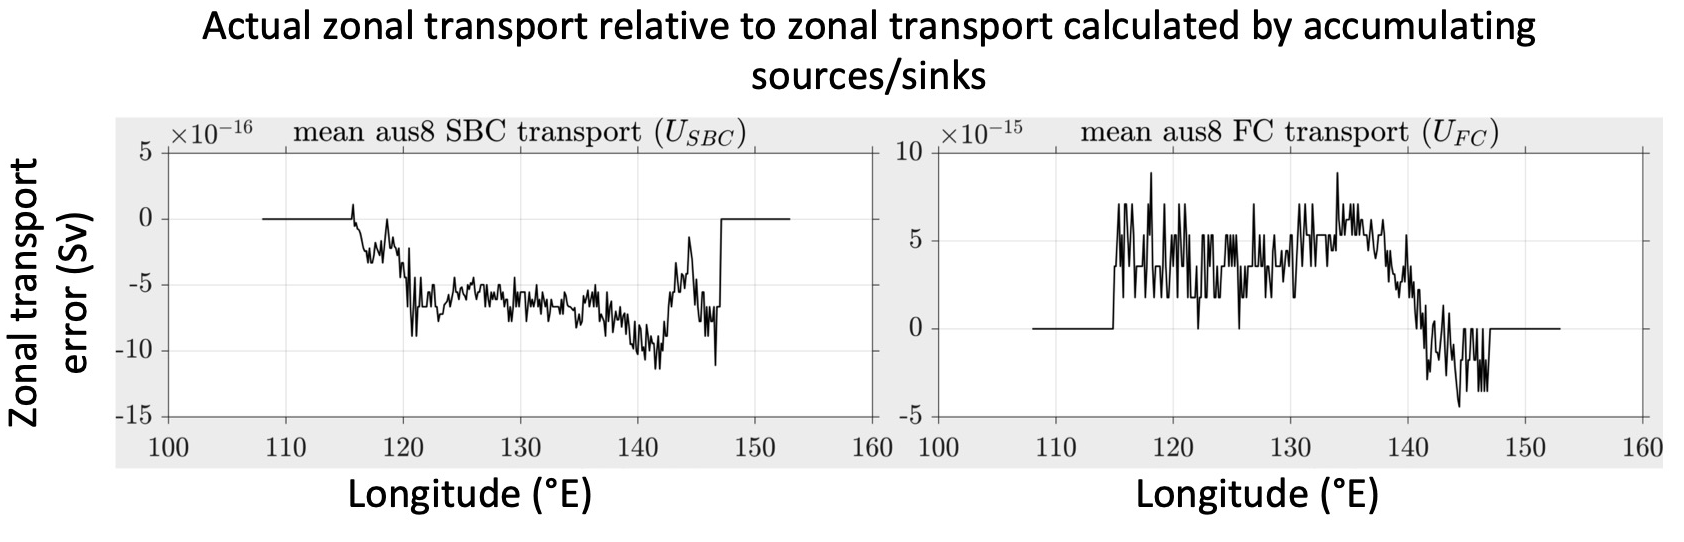
\includegraphics[width=1\textwidth, height=1\textheight, keepaspectratio]{Slide1_2.jpg}
    \caption{\label{Slide1_2}%
    Zonal transport error in Sv for the SBC (left) and the FC (right) showing the differences between the left-hand and right-hand sides of equations (16) and (17).}
\end{figure}

Since the volume budget closes to a high precision, it is evident that the longshore transport across a section can be determined by accumulating the lateral and vertical transports across the faces of the control volume upstream of the section, regardless of the orientation of the section (Fig.2).

\subsection{On using meridional sections rather than normal sections}
The most straightforward orientation of the section is meridional because the section then automatically follows faces of our classical lat-lon gridboxes. Next, we use Fig.\,\ref{slices} to explain the differences between meridional slicings and slicings normal to the coast.

\begin{figure}[hbp]
    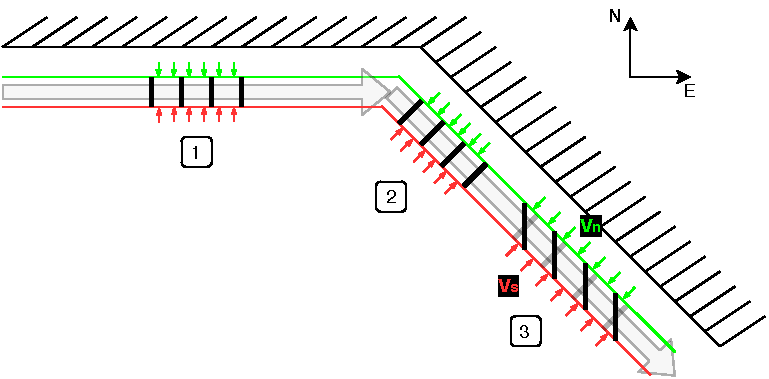
\includegraphics[width=1\textwidth, height=1\textheight, keepaspectratio]{slices.pdf}
    \caption{\label{slices}%
    Simplified schematics of the SBC (wide arrows) along a zonal shelf and a slanted shelf. The SBC is bounded to the north by the green line and to the south by the red line. The thin coloured arrows show the horizontal cross-boundary transports into the SBC across the north face ($V_n$) and south ($V_s$) of the SBC (we assume these transports to be into the SBC for simplicity). There is also an implied vertical transport across the bottom face of the SBC volume which we do not represent here for simplicity. $V_n$ and $V_s$ are the lateral transports across the north and south faces of the current, respectively. The slicing across the SBC volume is shown as thick lines. Case 1 shows meridional slices along a zonal shelf. Case 2 shows normal slices along a slanted shelf. Case 3 shows meridional slices along a slanted shelf (thick black lines) and normal slices along a slanted shelf (thick semi-transparent gray lines).}
\end{figure}

\subsubsection{On the difference between the zonal transport and the longshore transport}
Where the shelf is oriented zonally (Case 1 in Fig.\,\ref{slices}), the meridional slices are normal to the coast. If we were to slice the volume perpendicularly to the slanted coast (Case 2 Fig.\,\ref{slices}), this would result in a situation equivalent to Case 1. In Case 3 of Fig.\,\ref{slices}, meridional slices along the slanted coast (thick black lines) are longer than if they were normal to the coast (thick gray lines). Despite this difference, the volume transports across the two slices can be different only by lateral inflows across the sides of the little triangles formed by these two slices and by the vertical transports across the bottom faces of the triangles as shown below. In Fig.\,\ref{slices} and in the below equation we only consider the lateral inflows for simplicity.

If $\mathcal{\hat{U}}$ is the transport across the meridional slices and $\mathcal{U}$ is the transport across the slices normal to the coast, then

\begin{equation} \label{eq:20}
\mathcal{\hat{U}} = \mathcal{U} + V_{n}dl_{n} - V_{s}dl_{s},
\end{equation}
%
where $V_{n}$ is the inflow across the north face of the current (Fig.\,\ref{slices}), $dl_{n}$ is the length along the north face between a meridional slice and a normal slice, $V_{s}$ is the inflow across the south face of the current (Fig.\,\ref{slices}), $dl_{s}$ is the length along the south face between the meridional slice and the normal slice.

Hence, for a given meridional slice, some extra flows across the north face equivalent to $V_{n}dl_{n}$ are included in the current transport and some flows across the south face equivalent to $V_{s}dl_{s}$ are not included in the current transport, in comparison to a normal slice. When the current is wider, $dl_n$ and $dl_s$ become accordingly longer and the difference between $\mathcal{U}$ and $\hat{\mathcal{U}}$ tends to be larger (depending on the signs and sizes of $V_n$ and $V_s$).

\subsubsection{On the difference between zonal transport and longshore transport in the South Australian Current System case}
An implication of the above discussion is that, while it is true that volume transports with meridional slices will be different to volume transports with normal slices where the shelf is slanted, the difference between the meridional slicing and the normal slicing will be minimal provided:
%
\begin{itemize}
    \item that the slant is not too meridional. If the slant is too meridional, the sides of the little triangles (Case 3 in Fig.\,\ref{slices}) rapidly grow and the two volume transports ($\mathcal{U}$ and $\hat{\mathcal{U}}$) diverge; and
%
    \item that the currents are narrow. If the currents are too wide, the sides of the little triangles will also be too long.
\end{itemize}

In Fig.\,\ref{screenshot} we show a faded, zoomed-in version of Fig.\,3c where we added meridional and normal slices for the FC in a few selected regions. We can see that the triangles resulting from the tilt difference between meridional and normal slices increase in size where the current is wider (e.g.~western most slices) and where the slant is stronger (e.g.~eastern most slices). Given the narrowness of the SBC, the difference between meridional slices and normal slices will be minimal and is not shown in the figure. For the FC, there may be some local differences where the current gets wider or where the slant is stronger (west of Tasmania). These local differences are acceptable because in this paper we do not try to make precise comparisons of our transport values with other estimates at each point for the FC or SBC. Rather we intend to show how these currents' transports vary along the coast. Unless we compare our transport values directly with cross-shore observations, the difference $\mathcal{\hat{U}} - \mathcal{U} = V_{n}dl_{n} - V_{s}dl_{s}$ is immaterial because our volume budget analysis is self-consistent and leak-free. For all the reasons discussed above, we used the zonal transport for the transport of the currents.
%
\begin{figure}[tbhp]
\centering
    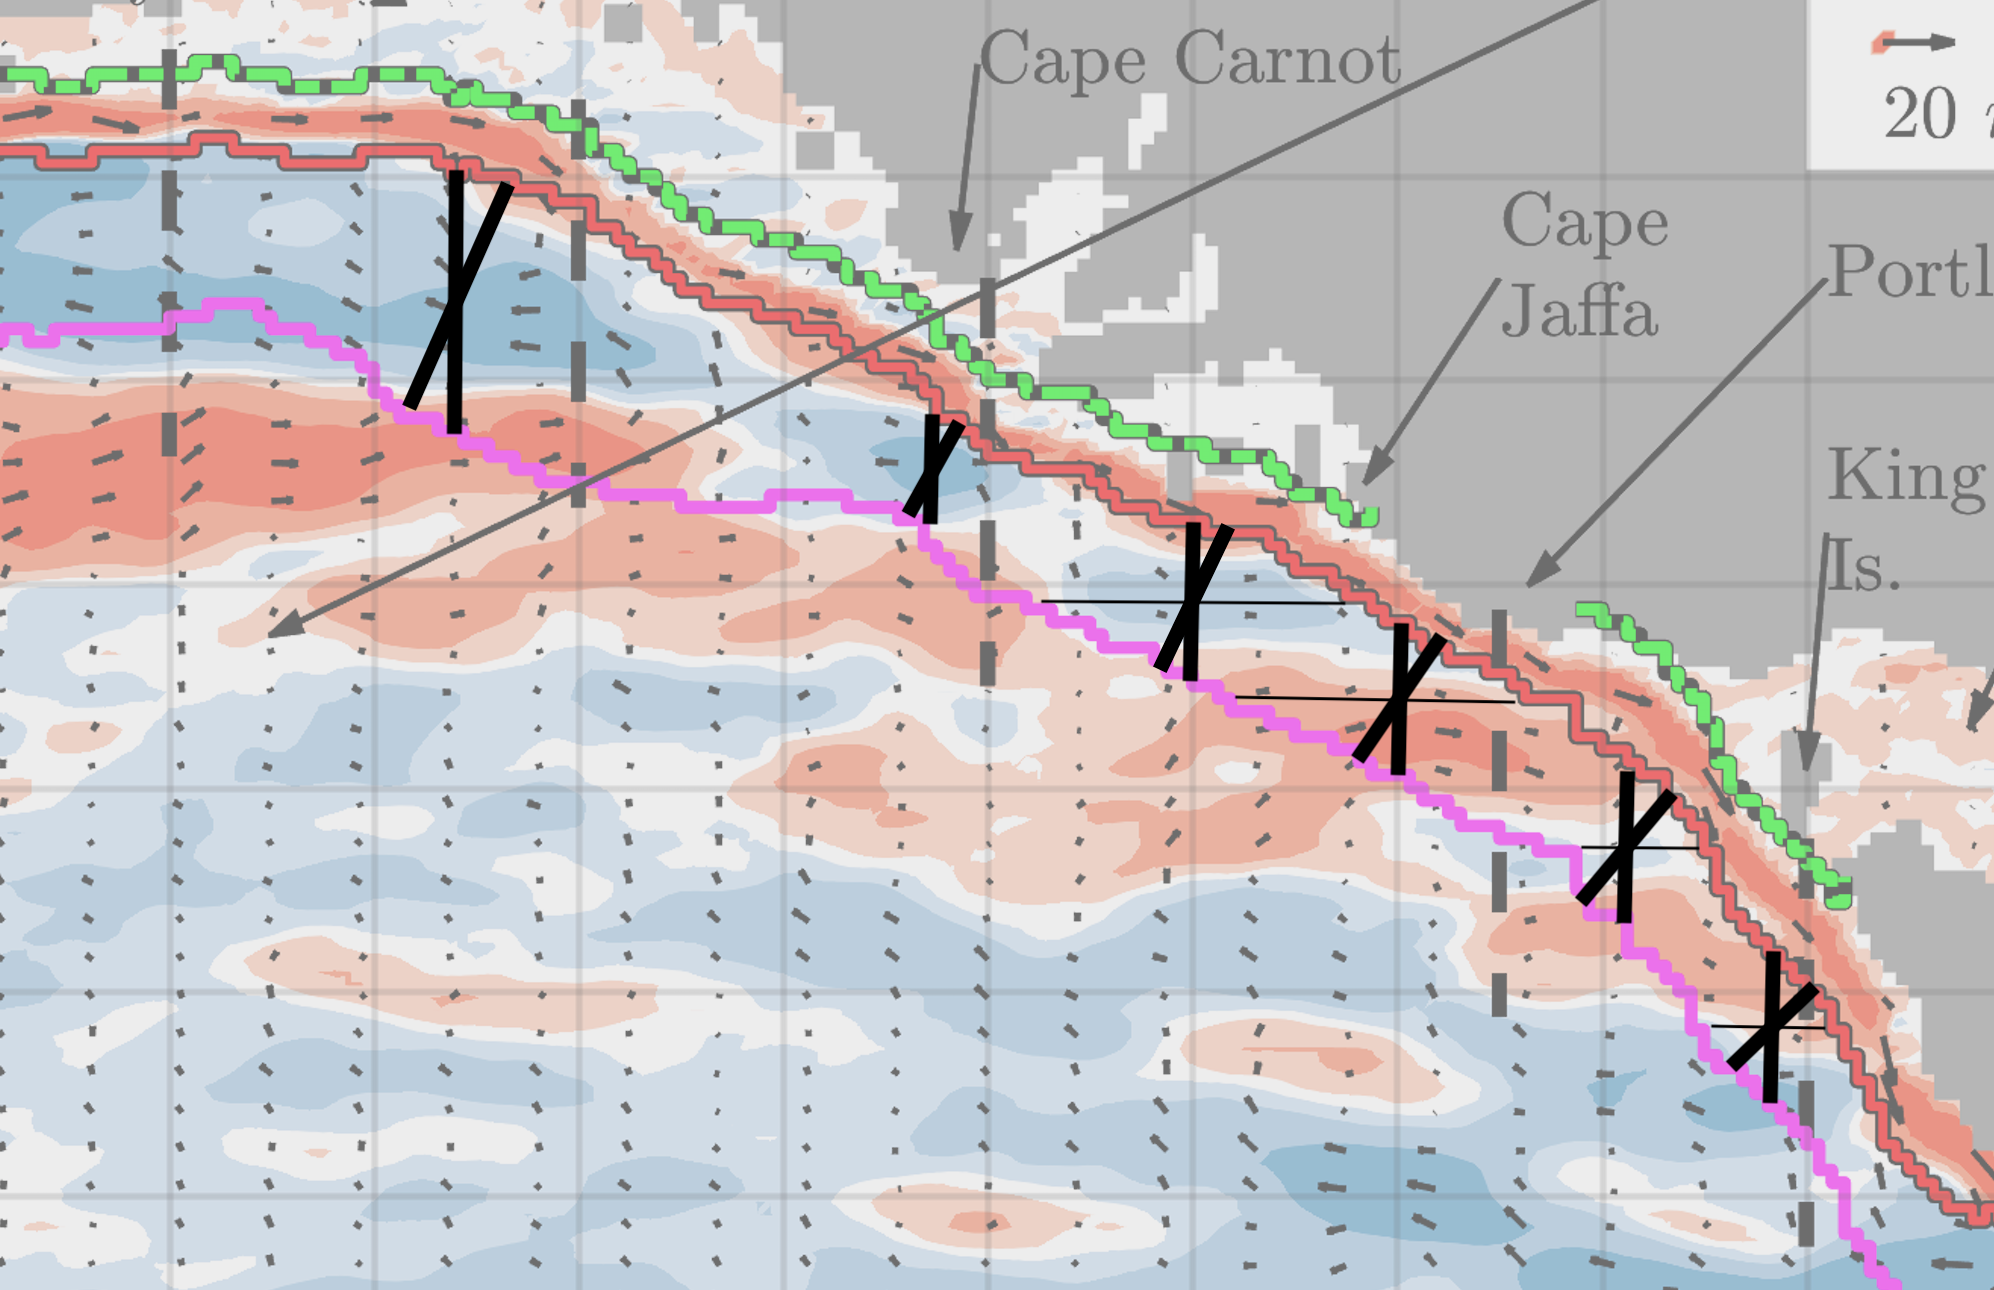
\includegraphics[width=0.8\textwidth, keepaspectratio]{screenshot_copy.png}
    \caption{\label{screenshot}%
    Faded and zoomed-in version of Fig.\,3c. Some examples of meridional and normal slices are shown as thick black lines. The difference between meridional slices and normal slices is shown by the triangles resulting from the tilt difference between the two slices. Zonal slices where the shelf is more slanted are shown as thin black lines. The normal slices are drawn by eye for illustrative purposes.}
\end{figure}

Even if we wanted to calculate a transport like $\mathcal{U}$ above, defining a cross-shore section is not straightforward given that the coast line is not a smooth curve. Then, if all sections follow outlines of grid-boxes, leak-free calculations are feasible, but in this case, each section would have to be defined manually. If, on the other hand, the sections are allowed to intersect grid-boxes, remapping the velocity field in such a way that the total volume is conserved would be very difficult and beyond the scope of this work. 

\clearpage
\bibliographystyle{agufull08.bst}
\bibliography{references.bib}

\end{document}